\chapter{Einleitung}

„Es gibt keine Norm für das Menschsein. Es ist normal, verschieden zu sein.“ (Weizsäcker 1993) 

Dieses aus einer Ansprache des ehemaligen Bundespräsidenten entnommene Zitat spiegelt den Leitgedanken von Inklusion wieder. Demnach alle Menschen mit augenscheinlichen Besonderheiten, jene mit befremdlichen Verhaltensweisen, mit Behinderungen, jene, mit denen die Kommunikation erschwert erscheint oder die in Armut leben, in die Gemeinschaft aufgenommen und von dieser bejaht werden sollen. 
Was aber diese 'schöne Idee', dass alle dazugehören und sich auch dazugehörig fühlen, konkret bedeutet und welche Konsequenzen sich daraus für die pädagogische Praxis ergeben, soll in dieser Arbeit hinterfragt werden.

Inklusion ist ein zentrales Anliegen der heutigen Zeit und eine sozial-ethische, eine politische und eine pädagogische Frage von gesamtgesellschaftlicher Größe. [Verstärkt in den Fokus öffentlicher Debatten ist Inklusion durch die UN-Behindertenrechtskonvention gerückt.]
Um das Thema in seiner Tragweite im Rahmen dieser Bachelorthesis bearbeiten zu können, wird 
sich die Inklusionsfrage auf den Elementarbereich, konkret auf den Kindergarten, beziehen. Verschiedene Autoren weisen auf das große Potential hin, das mit der Umsetzung von Inklusion im Kindergarten verbunden ist, da dort noch keine gleichgeschalteten Leistungen wie in der Schule erwartet werden, der Leistungs- und Konkurrenzdruck nicht im Vordergrund steht und weniger starke Exklusionsmechanismen wirken. Zudem wird inklusive Erziehungs- und Bildungsarbeit als wertvolles Ziel betrachtet, weil durch frühe Sozialisation, wenn Heterogenität bereits im Kindergarten gelernt und als positiv erlebt wird, ein gemeinsames Zusammenleben aller als normal erfahren werden kann und das wiederum die Voraussetzungen für ein neues gesellschaftliches Bewusstsein darstellt. Auch verbindet sich mit der Bereitstellung einer bestmöglichen Entwicklungsumgebung für alle Kinder die bildungspolitische Hoffnung, dass herkunftsbedingte Benachteiligung in Familien aus Armutslagen kompensiert werden können (vgl. Kron, Papke, Windisch 2010, Jerg 2011, Albers 2011). 

Der Begriff der Inklusion löst den der Integration ab. Mit dem Begriff der Integration wird nach Görannson (2010, 20) oftmals nicht mehr als die organisatorische Maßnahme der Platzierung des Kindes mit Behinderung in einer Gruppe mit Kindern ohne Behinderung verbunden. Inklusion fordert hingegen mehr als die Anpassung des Individuums an das bereits bestehende System. Laut Köhler (2009, 7) radikale Toleranz und den Verzicht auf die Enteignung individueller Lebensschicksale mit Verweis auf eine abstrakte Durchschnittsnorm. Eine erste Annäherung an den Begriff der Inklusion erfolgt durch Kron (2010, 15 f.). Sie definiert selbigen als Prozess, als kontinuierliches Bemühen, das darauf abzielt, ein angemessenes Umfeld für ’alle’ Kinder zu schaffen. Das hat Konsequenzen für die pädagogische Arbeit und bedeutet somit, dass alle Konzepte, Aktivitäten und Interaktionen an die unterschiedlichen Bedürfnisse, Interessen und Potentiale der Kinder anzupassen sind und gemeinsam mit ihnen, den Eltern und Fachkräften erarbeitet werden, nicht umgekehrt, wie bei der Zuweisung eines Integrationsplatzes häufig geschehen, dass sich die Kinder mit erhöhten Unterstützungsbedarf den im Vorfeld von ihnen unabhängig entworfenen Vorstellungen anzupassen haben.  

Obwohl Sarimski (2011, 4) auf die Statistiken der Kinder- und Jugendhilfe zu Tageseinrichtungen verweist und diese zeigen, dass etwa 75~\% der Kinder mit erhöhten Unterstützungsbedarf in Einrichtungen mit inklusiven Werten betreut werden und demnach die gemeinsame Erziehung und Bildung von Kindern mit und ohne Entwicklungserschwernisse mit großen Abstand am weitesten in den Einrichtungen des Elementarbereiches umgesetzt ist, muss festgehalten werden, dass wir bezüglich der Umsetzung inklusiver Werte in ihrer zuvor aufgezeigten Tragweite noch ganz am Anfang stehen. Mit Blick in die aktuellen Forschungsergebnisse ergibt sich ein ähnliches Bild. Laut Göransson (2010, 21) besteht die Herausforderung der Forschung darin einen Beitrag zur Entwicklung einer inklusiven Bildung und Erziehung zu leisten. Der Beitrag, der im Rahmen dieser Bachelorthesis geleistet wird, ist unter die Forschungsfrage gestellt: Unter Berücksichtigung welcher Aspekte ist Inklusion im Kindergarten umzusetzen?

\paragraph{Gang durch die Arbeit} 
Die vorliegende Arbeit ist in einen Teil A und einen Teil B gegliedert. Der Teil A umfasst die theoretischen und konzeptionellen Hintergründe inklusiver Erziehungs- und Bildungsarbeit im Kindergarten und umfasst die Kapitel 2 bis 4. Teil B unter Kapitel 5 beschreibt die qualitative Untersuchung, gefolgt von einer Zusammenfassung und Interpretation der Ergebnisse in Kapitel 6. Dem schließt sich eine Schlussbetrachtung und ein Ausblick in Kapitel 7 an sowie zuletzt das Literaturverzeichnis und der Anhang.

Da der Bezugsrahmen für die Umsetzung von Inklusion der Kindergarten ist, wird zuerst der Kindergarten als Erziehungs- und Bildungseinrichtung vorgestellt, erste Verweise auf Aspekte inklusiver Erziehung und Bildung werden hier bereits aufgegriffen.  
Zuvorderst wird die Entwicklung des Kindergartens von der Betreuungs- zur Bildungseinrichtung nach gezeichnet, um das Subsystem Kindergarten in Bezug zu dem Gesellschaftssystem zu stellen (Kapitel 2.1). Daran schließt sich die Darstellung der gesetzlich bindenden Grundlagen an, da bei der Frage nach der bestmöglichen Umsetzung von Inklusion im Kindergarten Richtlinien und geltende Bildungsempfehlungen der Bildungspläne im Auge behalten werden müssen (Kapitel 2.2).    
Im Folgenden (Kapitel 2.3) wird die Diskussion über das Selbstverständnis des Kindergartens fortgesetzt.
Da Inklusion nur unter der Wahrung von Qualitätsstandards umzusetzen ist, werden die für den Bereich der pädagogischen Qualität geltenden Qualitätsdimensionen aufgezeigt (Kapitel 2.4).

Erst in Kapitel 3 rückt Inklusion in den Vordergrund. Es erfolgt eine argumentative Begründung, warum die Umsetzung von Inklusion als ein sinnvolles und notwendiges Ziel anzusehen ist (Kapitel 3.1). Daran schließt sich die fachliche Debatte um die Begriffe Integration und Inklusion durch Alfred Sander (2004) an (Kapitel 3.2), gefolgt von dem Kapitel über die zu beachtenden Aspekte, die für die Umsetzung von Inklusion als notwendig erachtet werden (Kapitel 3.3).
 
Abschließend wird der aktuelle Forschungsstand aufgezeigt (Kap. 4).
   
Im zweiten Teil dieser Arbeit liegt der Fokus auf der qualitativen Untersuchung. Die Frage, welche Aspekte bei der Umsetzung von Inklusion zu berücksichtigen sind, wurden in Kapitel 3.3 theoriegeleitet beantwortet und werden nun mit Hilfe von Experteninterviews an der Praxis geprüft.
Kapitel 5.1 umfasst die Fragestellung und die Ziele der Studie sowie die Begründung der Entscheidung für ein qualitatives Design, konkret das Experteninterview. Daran schließen sich Ausführungen zum  Expertenbegriff und den befragten Experten an (Kapitel 5.2). Die Daten wurden mit Hilfe der Qualitativen Inhaltsanalyse ausgewertet (Kapitel 4.3). Daran schließt sich die Darstellung der Ergebnisse an (Kapitel 4.4.), gefolgt von der Deutung der Ergebnisse entlang der Theorie (Kapitel 4.5). [...] 

\part{Theoretischer Hintergrund}
\chapter{Der Kindergarten als Erziehungs- und Bildungseinrichtung in Deutschland}


„Vermutlich gibt es keinen Bereich des Erziehungs- und Bildungswesens, der sich in den letzten zwei, drei Jahrzehnten so grundlegend verändert hat und sich zugleich noch inmitten so umfangreicher Veränderung befindet wie die Kindertagesbetreuung“ (Hugoth 2010, 6).

Unter Kindertagesbetreuung werden laut Hugoth (2010, 5) alle Organisationsformen der Tagesbetreuung außerhalb von Schule und Familie zusammenfasst. Der Kindergarten -- das Untersuchungsfeld der vorliegenden Arbeit -- stellt mit einer bundesdurchschnittlichen Beteiligung von 95\,\% in Ostdeutschland und knapp 93\,\% in Westdeutschland (Stand: 2010, Bock-Famulla~\& Lange 2011, 9) das größte Kontingent innerhalb der Kindertageseinrichtung. Das bedeutet laut Honig, Joos ~\& Schreiber (2004, 12), dass der Kindergarten den größten Anteil an den Ausgaben für die Kinder und Jugendhilfe beansprucht und qualitativ mit der Grundschule vergleichbar ist. Dass der Kindergartenbesuch heute in Deutschland zur Normalbiografie eines Kindes gehört, ist nach Hugoth (2010, 8) auf den seit Januar 1996 bestehenden Rechtsanspruch auf einen Kindergartenplatz zurückzuführen. Dieser gilt für alle Kinder ab drei Jahren bis zum Ende des sechsten Lebensjahres. Nach Bock-Famulla~\& Lange (2011, 33) wird zudem angestrebt ab August 2013 den Rechtsanspruch auf einen Betreuungsplatz für alle Kinder vom vollendeten ersten bis zum vollendeten dritten Lebensjahr einzuführen. Im Zuge des bedarfsgerechten Ausbaus von Plätzen für Kinder unter drei Jahren, der momentan hohe politische Aufmerksamkeit erfährt, öffnet sich der Kindergarten auch für Kleinstkinder. Diese daraus resultierende erweiterte Altersspanne kann in der vorliegenden Arbeit jedoch nicht berücksichtigt werden.

Die Institution Kindergarten, dem Titel entsprechend, nur als Erziehungs- und Bildungseinrichtung zu beschreiben, greift zu kurz. Der Kindergarten hat den gesetzlichen Auftrag einer Trias zu erfüllen. Gemäß § 22 a SBG VIII (Gastinger~\& Winkler, 2009, 319) umfasst diese die Verantwortungsbereiche Bildung, Betreuung und Erziehung. Diese Arbeit beschränkt sich auf die Aspekte Bildung und Erziehung. 
Eine Annäherung an die beiden Begriffe schließt sich an: 

Auf die Frage, was bildet den Menschen, antwortet Hartmut von Hentig (2009, 13) mit der Gewissheit der Wahrheit selten nahe zu kommen: „Alles! -- Alles, selbst, wenn es langweilt oder gleichgültig läßt oder abschreckt. Dann ist dies die bildende Wirkung. Alles, weil der Mensch ein -- wundersam und abscheulich -- plastisches Wesen ist: veränderbar, beeinflussbar, reduzierbar, steigerungsfähig, auch gegen seinen Willen, gegen seine Einsicht, gegen seine Natur. [...] Anders als die übrige Kreatur ist [der Mensch] fast unbegrenzt auf Formung angelegt. Ist dies gewollt, nennt man sie Bildung.“ 
Hentig (2009, 15) bezeichnet den Begriff der Bildung als einen „verwickelten“ und „konturlosen“ Sachverhalt. Er verweist darauf, dass,  bisher keine gesamtgesellschaftliche Einigung hinsichtlich der Definition dieses Begriffes gefunden werden konnte, obwohl eine klar gefasste Definition für die Aufstellung von Richtlinien der Bildungspläne, für die Ausbildung der Erzieher und für die Einrichtung der Bildungsinstitutionen von enormer Bedeutung wäre. 
Ein zeitgemäßes Verständnis von Bildung, das als Konsens in der Bildungsdebatte gesehen werden kann, versteht Bildung laut Liegle (2003, 51) als umfassenden Prozess der Persönlichkeitsentwicklung, in dem das Kind in Auseinandersetzung mit der Umwelt tritt und ein  Bild von sich selbst und seiner Umwelt konstruiert. Unter dem Begriff der Erziehung wird demnach laut Hugoth (2009) die bewusste und zielgerichtete Beeinflussung des Kindes verstanden, die von den Erziehungsberechtigten und anderen Personen als seiner Persönlichkeitsentwicklung dienlich empfunden wird. Der Bildungs- und Erziehungsauftrag, speziell auf die Institution Kindergarten bezogen, findet seine Festlegung im Sozialgesetzbuch (vgl. Kapitel \ref{kap:AchtesSGB}). 

Das Eingangszitat beschreibt, dass wir gegenwärtig auf eine bereits stattgefundene und immer noch fortdauernde Phase des Umbruchs blicken. In dieser hat sich der Kindergarten als pädagogische Betreuungseinrichtung zur Bildungseinrichtung gewandelt und weites gehend etabliert. Im 12. Kinder- und Jugendbericht des Bundesministeriums für Familien, Senioren, Frauen und Jugend (2005, 28) wird beschrieben, dass sich im internationalen Vergleich für Deutschland ein Nachholbedarf ergibt, weil zu lange und zu einseitig Bildung ausschließlich von Seiten der Schule und Erziehung sowie Betreuung von Seiten der Familie erwartet und gedacht wurde. Von einem Umbruch, der den Kindergarten auf seinen Weg zur Bildungseinrichtung setzte, kann laut Nagel (2009, 12) seit Anfang der 90er Jahre gesprochen werden. Honig, Joos ~\& Schreiber (2004, 11) beschreiben, dass der Bildungsauftrag zwar schon seit der Bildungsdebatte der 70er Jahre als offiziell verankert galt, im Zuge der Wiedervereinigung beider deutscher Staaten und der damit verbundenen Vereinigung zweier sehr unterschiedlicher frühpädagogischer Erziehungssysteme jedoch erneute Auseinandersetzung erfuhr. Mit der Veröffentlichung der Ergebnisse der ersten PISA\footnote{PISA (Programme for International Student Assesement}-Studie im Jahre 2000 verließ die Bildungsfrage die Kreise der Fachleute und wurde zu einer gesamtgesellschaftlichen ausgeweitet.  

Laut Nagel (2009, 12) ist die aktuell intensiv geführte politische und fachliche Debatte über die Bedeutung, den Stellenwert und die Gestaltung frühkindlicher Bildungsprozesse Ausdruck des öffentlichen Bewusstseins, wie wichtig frühkindliche Bildung ist und welchen Einfluss pädagogische Arbeit auf die Entwicklung des Kindes nimmt. Bemühungen, wie sie Hugoth (2010, 6) aufzählt, die Qualifikation der pädagogischen Fachkräfte anzuheben, akademische Strukturen zu etablieren, und damit Rahmenbedingungen und die Qualität zu verbessern, zeigen das gewachsene öffentliche Interesse. Selbige tragen gleichzeitig dem Anspruch Rechnung, dass jedes Kind ein Recht auf Bildung hat. Im Mittelpunkt aktueller Bemühungen steht das Kind.   

Welche Aspekte und Notwendigkeiten den Wandel des Kindergartens zur Bildungseinrichtung hervorgerufen haben, soll in den folgenden Kapiteln (\ref{sec:kitaWandel} - \ref{sec:kitaSelbst}) aufgezeigt werden. 

\section{Der Wandel zur Bildungseinrichtung – was hat zu der veränderten Sichtweise beigetragen?}\label{sec:kitaWandel}
Die Notwendigkeit des Wandels ergibt sich einerseits aus den Ergebnissen, die von der PISA-Studie benannt worden sind, andererseits aus Erkenntnissen der Hirnforschung (vgl. Volkert 2008, Nagel 2009, Hugoth 2010, Schulz~\& Stammer 2011). Mit Hilfe der Hirnforschung konnte der hohe Stellenwert früher Bildungsprozesse abgesichert werden, womit sich insbesondere Hüther wissenschaftlich befasste. Als weiteren, durchaus fragwürdigen Aspekt bringen Schulz~\& Stammer 2011 sowie Ostner (2008) ‘Eltern als Risikofaktor‘ für die kindliche Entwicklung in die Debatte ein. Ostner (2008, 50 ff.) bezieht sich in ihrer Argumentation auf die Entwicklungstendenzen der Familienpolitik. 

\subsection{Die Ergebnisse der PISA-Studien}
Voran gestellt werden grundlegende Informationen über die Studie nach Prenzel, Carstensen, Frey, Drechsel~\& Rönnebeck (2007, 31-34). PISA ist eine internationale Untersuchung, in der Leistungen und Können von fünfzehnjährigen Schülern und Schülerinnen gemessen und verglichen werden. Die daraus gewonnenen empirischen Befunde dienen als Instrument zur Steuerung des Bildungssystems. Die PISA-Studie wird im Abstand von drei Jahren von der OECD (Organisation für wirtschaftliche Zusammenarbeit und Entwicklung) als Koordinator durchgeführt. Die Untersuchung konzentriert sich auf die Kompetenzbereiche Lesen, Mathematik und Naturwissenschaften und beabsichtigt nicht Lehrstoff abzufragen, sondern zu überprüfen, inwieweit Schlüsse aus Gelerntem gezogen und Wissen angewendet werden kann. Darüber hinaus wird der Zusammenhang zwischen Kompetenz und Merkmalen der sozialen und kulturellen Herkunft erfasst. Die daraus resultierenden Ergebnisse geben Auskunft darüber, inwieweit Kinder und Jugendliche aus unterschiedlichen sozialen Milieus vergleichbare und gerechte Chancen haben, im Bildungssystem die untersuchten Kompetenzen zu entwickeln. 
Laut Schulz~\& Stammer (2011, 7) waren die ‘beschämenden‘ Ergebnisse der ersten PISA-Studie im Jahre 2000 für Deutschlands Selbstverständnis als Bildungsnation erschütternd. Signifikant waren das schlechte Abschneiden von Migrantenkindern und die ungleichen Bildungschancen von Kindern aus bildungsfernen Familien. Laut dem Bundesministerium für Familie, Senioren, Frauen und Jugend (2005, 28) ist der Einfluss der sozialen Herkunft von Kindern auf ihre Bildungschancen in Deutschland so groß wie sonst nirgendwo. Auffallend schlecht schnitt Deutschland in den ersten beiden Testdurchläufen (in den Jahren 2000 und 2003) in dem Bereich der Lesekompetenz ab, was auf ein mangelndes Sprachverständnis zurückzuführen ist und sich ebenfalls auf die Bereich Naturwissenschaft und Rechnen auswirkte. Das knappe Fünftel der Schüler, die laut Bertelsmann-Studie (2010, 64) nicht richtig lesen können, stammt zum Großteil aus 'anregungsarmen' Familien. 
Daraus ergab sich laut Schulz~\& Stammer (2011, 8) die politische Forderung, die Qualifikation der Erzieherinnen durch die Akademisierung der Ausbildung zu erhöhen. Bock-Famulla~\& Lange (2011, 6) forderten zudem die Sprachförderung als zentral einzustufen und als Zielsetzung im Kindergarten zu verankern. Nach Hugoth (2010, 31) führten die Ergebnisse der PISA-Studie zu einer grundlegenden, alle Bildungsbereiche umfassenden, Bildungsreform.
 
\subsection{Erkenntnisse der Hirnforschung}
Neurobiologische Erkenntnisse, die durch bildgebende Verfahren, so genannte funktionelle Kernspintomographie, ermöglicht wurden
belegen laut Hüther (2011, 46 f.), dass die genetischen Programme, die für die Steuerung der Hirnentwicklung zuständig sind und unser Denken, Fühlen und Handeln in Form von Verschaltungen hervorbringen, sich dadurch auszeichnen, dass sie „so wenig wie möglich festlegen“. Daraus resultiert ein veränderungsfähiges, zeitlebens lernfähiges Gehirn, dessen Struktur sich durch die im Laufe des Lebens gemachten Erfahrungen entwickelt. Er entlarvt die lange Zeit geltende Vorstellung, dass der Prozess der strukturellen Ausreifung des Gehirns gegen Ende des dritten Lebensjahres als weitgehend abgeschlossen anzusehen ist, als Irrtum. Das Gehirn mit seiner großen Plastizität ist kontext- und nutzungsabhänig. Wie sich Kinder entwickeln, hängt also im entscheidenden Maße davon ab, womit sie sich intensiv beschäftigen und wozu sie in Interaktionsprozessen angeregt werden. Ohne lebendige Interaktionen würden Neugeborene überhaupt nichts und das Kindergartenkind nur sehr wenig lernen können. Neurobiologische Erkenntnisse belegen auch, dass die Aufnahme und Verankerung neuer Informationen im Gehirn stark beeinträchtigt wird, wenn das Kind Angst hat oder unter Druck steht. Sicherheit und Vertrauen sind deshalb wichtige Voraussetzungen für Lernprozesse. Zu den lern- und entwicklungsförderlichen Bedingungen gehört neben der Anregung deshalb 
auch eine sichere Bindung. Qualitäten wie Einfühlungsvermögen, Vertrauen und Anerkennung der verantwortlichen Erwachsenen bilden demnach die Basis, dass das Kind auf Entdeckungsreise geht und Neuentdecktes auch verarbeiten kann.
Becker-Stoll (2009, 46) bringt es auf einen einfachen Nenner: „Ohne Emotion keine Kognition und ohne Bindung keine Bildung.“

Die nach Hüther (2011, S. 47) zu frühen Zeitpunkten geformten neuronalen Netze stehen stärker mit emotionalen Zentren in Verbindungen und sind deshalb stabiler herausgebildet als später entstandene Netzwerke. Spätere sind im besonderen Maße modellierbar.
 Weil der emotionale Eindruck ein so nachhaltiger ist, gleicht das Bild vom Kind, das in die Schule kommt dem eines „fertigen“ kleinen Menschen. Auch wenn Lernprozesse nicht als abgeschlossen betrachtet werden dürfen, gilt, dass das menschliche Gehirn im Wesentlichen durch die Erfahrungen strukturiert wird, die es in der Phase seiner Hirnentwicklung macht. 
Diese Phasen, die mit struktureller Veränderungen und einer messbaren Volumenzunahme einhergehen, sind von der Geburt bis zum 12. Lebensjahr und erneut zu Beginn der Pubertät zu beobachten. 
Einerseits ist der Mensch mit einem derart offenen und lernfähigen Gehirn ausgestattet, andererseits werden in der Vorschulzeit Weichen gestellt, die später schwer zu verstellen sind, vor allem im Hinblick auf Bindung und das Erlernen der Sprache.
In jedem Fall aber gilt, dass Kinder als aktiv Lernende zu begreifen sind und deshalb „als bildungsbedürftig und bildungswillig und als Bildungssubjekte verstanden werden müssen“ (Hugoth 2010, 31).
 

\subsection{Eltern als Risikofaktor für die kindliche Entwicklung}\label{sec:Risikofaktoren}
Schulz~\& Stammer (2011, S. 7) tragen als weiteres Argument zu dieser Diskussion bei, dass Familien in der Öffentlichkeit zunehmend unter einer Defizitperspektive betrachtet werden. Gründe dafür sehen sie vor allem in der medialen Berichterstattung, in welcher die riskante Lebenswelt der Kinder dargestellt wird durch zu viel Medienkonsum, häusliche Gewalt und Missbrauch, Drogenkonsum, Ehescheidungen und zu wenig Schulabschlüsse. Laut der Bertelsmann-Studie (2009) verließen im selbigen Jahr 58400 Jugendliche die Schule ohne Abschluss. 

Ostner (2008, 59) nimmt eine radikale Perspektive hinsichtlich der familienpolitischen Entwicklung der letzten Jahrzehnte ein. In ihrer Bestandsaufnahme bezieht sie sich auf ? (Quellen). Sie verweist darauf, dass aus Expertensicht heute viele Menschen als insuffizient in Fragen der Erziehung angesehen werden. Wenn die Familien nicht mehr den Schutz- und Förderraum für die Erziehung der Kinder bieten können, ist die Solidarität der Gemeinschaft gefragt beziehungsweise muss die Verantwortung für die Bildung der Kinder in professionelle Hände gegeben werden. Nach Ostner (2008, 58) wird das durch PISA aufgedeckte deutsche Bildungsversagen als Versagen der Familie beziehungsweise in letzter Konsequenz als Versagen des Staates interpretiert: „Er hat bisher unterlassen durch möglichst frühe Entfamilisierung des Kindes die Vererbung des Bidungsmisserfolges zu verhindern“ (Ostern 2008, 58). Ostner (2008, 50) unterscheidet begrifflich zwischen „Familisierung“ und „Entfamilisierung“ als zentrale Elemente der Familienpolitik. Familisierung stärkt die Familie und setzt auf das Verständnis, dass Frauen 'nur' Mütter sein sollen. Entfamilisierung bedeutet, dass die Aufgaben aus der Familie herausgelöst und durch Übergabe an Kindertagesstätten professionalisiert werden sollen. Die Frau soll gemäß ihres neuen Rollenverständnis auf jeden Fall erwerbstätig sein, aber möglichst auch Kinder haben. Der propagierte Weggang vom Familismus ist laut Ostner (2008, 57 f.) vor allem für Westdeutschland neu, da hier die mütterliche Kleinkindbetreuung bis heute weit verbreitet ist. Im europäischen Vergleich stellt Westdeutschland jedoch eher die Regel und nicht die Ausnahme dar. Das Erhöhen der Erwerbsbeteiligung von Müttern dient vor allem arbeitsmarktpolitischen Zielen: Armutsprävention der Kinder und  Konsumsteigerung. 
Durch das Reduzieren der elterlichen Aufgaben durch frühe Institutionalisierung der Kinder wird mehr Vereinbarkeit mit den Anforderungen des Arbeitslebens erreicht. Folgt man Ostners Argumentation (2008, 51), hat sich in Deutschland ein Paradigmenwechsel von Familisierung zu Entfamilisierung ereignet. Aktuelle familienpolitische Reformen zielen darauf ab, Betreuung, Bildung und Erziehung früh und nachhaltig aus der Familie herauszulösen. Das Ziel, gleiche Qualität und Chancen für alle Kinder, soll durch Ganztagsbetreuung, durch den Ausbau von Plätzen für Kinder unter drei Jahren und durch das politische Forcieren einer 'beschäftigungsfreundlichen Familie' erreicht werden. Die Vorbereitung des familienpolitischen Paradigmenwechsels erfolgte laut Ostner (2008, 58) durch die Rede von zweierlei Risiken: Zum einen potentielle Kinderarmut, bedingt durch die Bildungsferne der Eltern und durch unzureichende Ausschöpfung des Erwerbspotentials der Frau, wenn sie als Mutter eingebunden ist, zum anderen die Darstellung der Eltern als Risikofaktor oder Gefahrenzone. 

Die Autorin der hier vorliegenden Arbeit sieht die familienpolitische Einbettung als wichtig an, weil durch das Aufzeigen, dass nicht familien-, sondern wirtschafts- und arbeitsmarktpolitische Zielsetzungen vordergründig sind, Familienversagen kritisch zu hinterfragen ist. Was Familien leisten können und sollen, wird politisch forciert.
 
Honig et al. (2004, 12 f.) schreiben, dass „scheinbar getrennt von der Debatte um den Bildungsauftrag“ seit den 80er Jahren eine sozialpolitische Diskussion um die Vereinbarkeit von Familie und Beruf stattfindet. Später wurde die Diskussion um das Thema Armut von Kindern erweitert. Die Debatte wird stark von der Politik der Europäischen Union und der OECD beeinflusst und steht in den komplexen Prozessen um die Neustrukturierung des Wohlfahrtstaates. Auch hier lassen sich die Aspekte wie „Mobilisierung der Beschäftigungsfähigkeit der Frau“ wiederfinden, genauso wie demographische Probleme einer zunehmend alternden Gesellschaft, auf die pro Familie im Durchschnitt nur 1,3 Kinder (Stand: ) fallen. Der Fünfte Familienbericht von 1994 nimmt die so genannte 'Zukunft des Humanvermögens' in den Blick -- die Qualifizierung des kostbaren Nachwuchses. Der Elfte Kinder- und Jugendbericht von 2002 stellt die Frage nach dem Verhältnis von öffentlicher und privater Verantwortung und weist Kindertagesstätten eine Dienstleistungsfunktion zu. „Auch im Kontext dieser Dienstleistungsfunktion geht es um Bildung; aber sie hat weniger die Bedeutung einer Chance zur Persönlichkeitsentwicklung oder die eines schulisch vermittelten Wissens als die eines Bürgerrechts oder einer Investition in das Humanvermögen, welche in einem engen Wechselverhältnis steht zu familien-, frauen-, arbeitsmarkt- und sozialpolitischen Funktionen des Betreuungssystems“ (Honig et al. 2004, 12).  
 
Vor dem Hintergrund dieses Paradigmenwechsels und der komplexen Veränderungen sind die Fragen, was einen guten Kindergarten ausmacht, was dieser leisten sollte und in wessen Dienst dieser gestellt wird, um so dringender. Ist ein guter Kindergarten einer, der den Kindern zu der Entfaltung ihrer individuellen Möglichkeiten verhilft und sie auf die kommenden Herausforderung der Lebens- und Arbeitswelt vorbereitet? Ist es einer der den Sinn für Fairness und Respekt stärkt und zu gerechten Lebensverhältnissen beiträgt, indem er Minderheiten integriert? Ist es einer, der Familien unterstützt und beides,  Erwerbstätigkeit und Familienleben, ermöglicht? Ist es einer der das Humanvermögen unserer Gesellschaft mehrt? 

\subsection{Berührungspunkte zwischen Bildungs- und Inklusionsdebatte}

Nach Honig et al. (2004, 12 f.) wurde die integrationspolitische Funktion des Betreuungssystems lange Zeit übersehen. Erst mit den Ergebnissen der ersten PISA-Studie wurde offensichtlich, dass Kinder mit Migrationshintergrund in der deutschen Gesellschaft benachteiligt werden. In aktuellen Diskursen wird das Ziel benannt, gleiche Qualität und gleiche Chancen für alle Kinder herzustellen. Dieses egalitäre Ziel erfordert folgerichtig bedingungslose Teilhabe aller Kinder, das heißt inklusive Bildung. Laut Jerg (2011, 47) sind die inklusiven Bestrebungen der Behindertenrechtskonvention – in Artikel 24 der Konvention wird unmissverständlich eine inklusive Bildung auf allen Ebenen gefordert – anschlussfähig an aktuelle Diskurse über Bildungsungleichheit und Chancengerechtigkeit. Ob in der von Ostner (2008, 50) dargestellten familienpolitischen Bildungsdebatte aber wirklich und uneingeschränkt alle Kinder gemeint sind, bleibt fraglich. Einigkeit herrscht laut Ostner (2008, 59) darüber, dass die Chancen 'bildungsferner' Kinder oder Kinder mit nicht-deutscher Muttersprache erhöht werden können, wenn diese engen Kontakt mit deutschen 'bildungsnahen' Kindern haben. Jerg schreibt (2011, 47), dass neben Behinderung weitere Differenzkategorien wie sozialer Status, Armut, Migrationsgeschichte im Inklusionsverständnis berücksichtigt werden (vgl. Kapitel ?). Die Annahme, dass die aktuell geführte Bildungsdebatte auch eine Inklusionsdebatte ist, liegt nahe, trifft aber nur bedingt zu. Stellen wir die Darstellungen von Ostner und Jerg gegenüber, werden unterschiedliche, geradezu gegensätzliche gesellschaftliche Interessen deutlich: Die Inklusionsbestrebungen zielen darauf ab, dass Bildung im Sinne von Jerg als Menschenrecht anerkannt wird und jedem Menschen ohne Ausnahme uneingeschränkter Zugang zu Bildung zugestanden wird. Dem gegenüber steht die Bildung nach Ostner, die unter ökonomischen Gesichtspunkten eine viel versprechende Ressource darstellt. In diesem Sinne ist Bildung kein Zugeständnis oder Geschenk, sondern mit einer Erwartungshaltung verbunden: das Kind soll mit Bildung so ausgestattet sein, dass es ich als Erwachsener in die Gesellschaft einbringt und einen hohen Wert an wirtschaftlichen Kapital vorzuweisen hat. Menschen mit Behinderung oder besonderem Förderbedarf haben jedoch nur eingeschränkt die Möglichkeit sich einzubringen. Ethisch ist die Haltung vom Menschen als Humankapital in keiner Weise zu rechtfertigen. Der Mensch darf nicht an einen Zweck gebunden sein. Nach Spaermann (2011) ist die Würde des Menschen dann verletzt, wenn es offen oder stillschweigend heißt, auf ihn kommt es nicht an. 

Jerg (2011, 51) verweist auf Andreß~\& Stichweg, wonach Startpunkte für Exklusionskarrieren an Barrieren zur Bildung und Armut festzumachen sind. Diese wiederum werden durch das Etikett 'Behinderung' oder durch andere Benachteiligungen beschleunigt. Mögliche Stoppmechanismen in der Exklusionskarriere sind beispielsweise Gesetze, welche die Teilhabe an den allgemeinen Bildungseinrichtungen garantieren. Das begründet auch, warum laut Jerg (ebd.) die UN-Behindertenrechtskonvention zum Hoffnungsträger für Familien mit Kindern mit Unterstützungsbedarf wird. 

\section{Gesetzliche Grundlagen und Orientierungshilfen für die Arbeit im Kindergarten unter Berücksichtigung von Inklusion}

In diesem Kapitel werden zweierlei Anliegen verfolgt. Zum einen sollen die allgemeinen das Untersuchungsfeld Kindergarten beschreibenden gesetzlichen Grundlagen sowie normativen Bezüge aufgezeigt werden. Zum anderen soll die Frage geklärt werden, inwiefern diese dem Anspruch inklusiver Bildung und Erziehung gerecht werden. 

In Deutschland gilt der Kindergarten nach Kron, Papke~\& Windisch (2010, 103) als Elementarbereich des Bildungswesens, ist aber bedingt durch die deutsche Entwicklungsgeschichte nicht dem Schulsystem, sondern als ein eigenständiger Bereich dem Sozial- und Jugendhilfesektor zugeordnet. 
Gesetzliche Grundlage für die Arbeit in Kindergärten ist nach Hugoth (2010, 23) hauptsächlich das Achte Buch des Sozialgesetzbuches (SGB VIII), das sogenannte Kinder- und Jugendhilfegesetz (KJHG). Näheres zum Inhalt und Umfang der Aufgaben und Leistungen bezüglich der Förderung von Kindern lässt sich den jeweiligen Ländergesetzen der Bundesländer finden. Auf diese kann jedoch in der vorliegenden Arbeit aus Platzgründen nicht eingegangen werden. Inwiefern die UN-Kinderrechtskonvention zur gesetzlichen Grundlage pädagogischen Handelns gehört, kann diskutiert werden. Laut dem Ministerium für Kultus, Jugend und Sport Baden-Württemberg (2011) bilden sowohl das SGB VIII als auch die UN-Kinderrechtskonvention die gesetzlichen Grundlagen des Kindergartens. Dem entsprechend wird in der vorliegenden Arbeit die UN-Kinderrechtskonvention zu den allgemeinen gesetzlichen Grundlagen gezählt. 
Als weitere normative Bezugsgröße werden die Bildungspläne der Bundesländer vorgestellt. Nach Nagel~\& Becker-Stoll (2009, 8) stehen  mittlerweile allen Bundesländern Bildungspläne zur Verfügung, welche als differenzierte Orientierungshilfe für das pädagogische Handeln dienen. Jedoch ist deren Verbindlichkeit laut Nagel (2009, 198 f.) von Bundesland zu Bundesland verschieden. In Bayern, Berlin, Sachsen und Thüringen ist die Orientierung am Bildungsplan gesetzlich bindend, während dessen in allen anderen Bundesländern lediglich Vereinbarungen zur Umsetzung mit den Trägern getroffen werden.
 
Nach Darstellung der Rahmeninhalte des SGB VIII, der Kinderrechtskonvention sowie der Bildungspläne schließt sich die Auseinandersetzung an, inwiefern diese Dokumente inklusive Tendenzen aufweisen. 

Die UN-Behindertenrechtskonvention als der wichtigste Bezugspunkt für die inklusive Arbeit im Kinderarten wird erst in Kapitel~\ref{sec:BRK} vorgestellt, da laut Albers (2011, 14) Inklusion innerhalb der pädagogischen Arbeit noch lange keine Selbstverständlichkeit darstellt und deswegen nicht zu den gesetzlichen Grundlagen gezählt werden kann. 

\subsection{Das Achte Sozialgesetzbuch (SGB VIII)}\label{kap:AchtesSGB}

Nach Nagel (2009, 194) ist der Bildungs-, Erziehungs- und Betreuungsauftrag seit 1990 gesetzlich festgeschrieben. Inhalte frühkindlicher Bildung und Betreuung und ihre Aufgabenbeschreibung für die pädagogische Fachkraft werden in § 22 und § 22a SGB VIII geregelt. 
In § 22 Abs. 2 SGB VIII wird nach Kunkel (2006, 251) der allgemeine Zielhorizont für die Förderung beider Angebotsformen festgelegt. 
„Tageseinrichtungen für Kinder und Kindertagespflege sollen:

\begin{enumerate}
\item die Entwicklung des Kindes zu einer eigenverantwortlichen und gemeinschaftsfähigen Persönlichkeit fördern,
\item die Erziehung und Bildung in der Familie unterstützen und ergänzen,
\item den Eltern dabei helfen, Erwerbstätigkeit und Kindererziehung besser miteinander vereinbaren zu können“ (Gastiger~\& Winkler, 2009, 319).  
\end{enumerate}

Der in § 22 Abs. 3 SGB VIII (ebd.) inhaltlich konkretisierte und die Trias Erziehung, Bildung und Betreuung umfassende Förderungsauftrag ist ein ganzheitlicher und individualisierter. Dies drückt sich aus, in dem die soziale, emotionale, körperliche und geistige Entwicklung des Kindes in den Blick genommen und sich an den jeweiligen individuellen Bedürfnissen und Interessen des Kindes sowie an seinem Alter und Entwicklungsstand, den sprachlichen und sonstigen Fähigkeiten und der Lebenssituation orientiert werden soll. Des Weiteren soll die kulturelle Herkunft des Kindes Berücksichtigung finden. Der Förderungsauftrag schließt die Vermittlung von Werten und Regeln ein. Nach Kunkel (2006, 251) wird mit der Entscheidung, die Kindertagesstätten im Rahmen der öffentlichen Hilfen zu belassen und auszubauen, statt sie wie auch die Schulen in Bildungsverantwortung der Länder zu übergeben, der „Charakter der Elementarerziehung als grundlegende Förderung der individuellen Persönlichkeitsentwicklung“ (Kunkel, 2006, 251) hervor gehoben. Dieser kindzentrierte Anspruch ist eng mit der elterlichen Erziehungsverantwortung verknüpft, weshalb im gesetzlichen Bezugskontext die Förderung von Kindern als Ergänzung der elterlichen Erziehung zu lesen ist. 

In diesem Sinne sind die pädagogischen Fachkräfte nach § 22 a Abs. 2 Satz 1 Nr. 1 zur Zusammenarbeit mit den Eltern verpflichtet. Dabei sollen nach Kunkel (2006, 257) Brüche im pädagogischen Handeln vermieden werden, so dass eine Kontinuität des Erziehungsprozesses abgesichert ist. Dafür Sorge zu tragen, dass eine auf das einzelne Kind bezogene Zusammenarbeit stattfindet, verlangt, dass der Träger für diese anspruchsvolle Elternarbeit ausreichend Zeit einräumt und den pädagogischen Fachkräften Unterstützung zukommen lässt. Über die Elternarbeit hinaus soll nach § 22a 2 Satz 1 Nr. 2 ebenso Vernetzung mit kinder- und familienbezogenen Institutionen und helfenden Diensten, zum Beispiel Familienberatungsstellen, und zuletzt Schulen sicher gestellt werden. Nach Kunkel (ebd.) ist die Öffnung zu den genannten Einrichtungen Ergebnis der Bestrebungen eine kommunale Infrastruktur für Familien und Kinder zu schaffen und ein „sozialraumbezogenes integriertes Jugendhilfeangebot“ (Kunkel 2006, 257) zu installieren. Ergänzend werden in § 22a Abs. 1 SBG VIII qualitätssteuernde Vorgaben gemacht. Die Träger der öffentlichen Jugendhilfe haben demnach nach Kunkel (2006, 256) den Auftrag für gute Qualität der Einrichtungen zu sorgen. Qualität misst sich am Erarbeiten eines Konzepts, am Anwenden von Verfahren zur Evaluation der pädagogischen Arbeit und an Qualitätsfaktoren wie zum Beispiel der Zusammenarbeit mit den Eltern der betreuten Kinder.

Da nach Art. 6 Abs. 2 S. 1 Grundgesetz sowie § 1 Abs. 2 SBG VIII die Pflege und Erziehung der Kinder das natürliche Recht der Eltern und die zuvorderst ihnen obliegende Pflicht ist, gilt es, wie bereits geschildert, sich an den Bedürfnissen der Kinder und Eltern zu orientieren und Eltern in allen wesentlichen Angelegenheiten mit einzubeziehen. In Art. 6 Abs. 2 Satz 2 und § 1 Abs. 2 steht weiter, dass über die Betätigung der Eltern die staatliche Gemeinschaft wacht. Hierin drückt sich nach Kunkel (2010, 41) das Wächteramt des Staates aus. Um den Schutz des Kindeswohls zu erhöhen, wurde nach Hugoth (2010, 24) im Jahre 2005 das Kinder- und Jugendhilfeerweiterungsgesetz   verabschiedet und im Zuge dessen § 8a „Schutzauftrag bei Kindeswohlgefährdung“ neu im SBG VIII aufgenommen. Mit dem Auftrag gemäß § 8a (2) SGB VIII, dass die Träger von Einrichtungen den Schutzauftrag wahrnehmen und über das Wohl der Kinder wachen sollen, sind sie, laut Hugoth (2010, 32), in die Verantwortung des staatlichen Wächteramtes mit einbezogen. Nach Kunkel (2010, 41f) ist damit eine gesichterte Rechtsgrundlage für das Handeln der Fachkräfte und ein entsprechender „Fahrplan“ geschaffen, der aufzeigt, wie das Jugendamt zu verfahren hat, wenn es Hinweise auf eine Kindswohlgefährdung erhält. Demnach sind pädagogischen Fachkräfte gefordert, „gewichtige Anhaltspunkte“, die nach § 8a (1) SGB VIII für die Gefährdung des Wohls eines Kindes sprechen könnten, zu erkennen und auf Verdacht weitere Fachkräfte zur Abschätzung des Risikos hinzuzuziehen. Kunkel (2010, 49) definiert gewichtige Anhaltspunkte als Tatsachen, die generell, bei ungehindertem Geschehensablauf mit hoher Wahrscheinlichkeit in absehbarer Zeit einen schwerwiegenden und dauerhaften Schaden im Sinne von § 1666 BGB \footnote{Nach Kunkel (2010, 42) sind gewichtige Anhaltspunkte nach § 1666 BGB zum Beispiel körperliche oder seelische Misshandlung, Verweigerung notwendiger ärztlicher Maßnahmen, Nicht-Erfüllung der Schulpflicht, Verleitung zu Kriminalität und Prostitution.} bewirken würden. Nach Kunkel (2010, 43) besteht die Funktion des staatlichen Wächteramtes nicht darin, das Beste für das Kind zu erreichen, sondern das Schlimmste zu vermeiden.

\subsection{Die UN-Kinderrechtskonvention}

Nach Köpcke-Duttler (2011, 17) ist das Übereinkommen über die Rechte des Kindes vom 20. November 1989 ein völkerrechtliches Abkommen, in welchem sich die Vertragsstaaten verpflichten, die in der Konvention benannten Rechte jedem Kind ohne jegliche Diskriminierung zu gewährleisten. Das Abkommen ist laut Hugoth (2011, 8) 1992 von Deutschland ratifiziert worden. Das bedeutet, dass sowohl die Bundes- und Landesregierung wie auch die Akteure der Kinder-, Jugend- und Behindertenhilfe, zu denen auch die Träger der Kindertagesstätten gehören, sich verpflichten, diese Rechte nachweislich umzusetzen. Um Kinder aufgrund ihrer Hilfsbedürftigkeit und Abhängigkeit vor Gefährdungen zu schützen, werden sie im Rahmen der UN-Deklaration als eigenständige Persönlichkeiten anerkannt und mit spezifischen Grundrechten ausgestattet. Zu diesen zählen unter anderen das Recht auf personale Selbstbestimmung, auf Schutz vor jeder Art von Gewalt und Misshandlung, auf Gesundheit, Bildung und Förderung sowie auf Partizipation\footnote{Bezogen auf Prozesse der Bildung und Erziehung bedeutet Partizipation laut Hansen, Knauer~\& Sturzenhecker (2011, 19): „Entscheidungen, die das eigene Leben und das Leben der Gemeinschaft betreffen, zu teilen und gemeinsam Lösungen für Probleme zu finden“. Was Partizipation für den Umgang mit Kindern konkret heißt, bedarf laut Hansen et al. (2011, 25) gründlicher Überlegungen und aktiver Unterstützung seitens der Bezugs- oder Betreuungspersonen, so dass das Kind beteiligungs- und entscheidungsfähig wird. Grundsätzlich gilt Kinder zu fragen, was sie wollen, ihre Wünsche zu berücksichtigen, sich für sie Zeit zu nehmen und ihnen zuzuhören. Darüber hinaus ist das, was ein Kind braucht, um wirklich mitentscheiden zu können, sehr unterschiedlich. Manchen fehlt es an Informationen, anderen an alternativen Erfahrungen, wieder anderen an verbalen Ausdrucksmöglichkeiten oder Mut, um eine Entscheidung treffen zu können.}. 
Artikel 12 der Kinderrechtskonvention sieht vor, dass die Meinung des Kindes angemessen und entsprechend seinem Alter und seiner Reife berücksichtigt wird, auch vor Gericht. Nach Hansen, Knauer~\& Sturzenheckeret (2011, 9) können diese spezifischen Rechte nicht in eigener Regie von Kindern wahrgenommen werden. Dafür bedarf es verantwortungsbewusster Erwachsener, die sie individuell begleiten, sie unterstützen und auch einen Teil ihrer Macht aufgeben. Da Kinder über eigene Rechte verfügen, haben Erwachsene nicht mehr das Monopol über das Kind zu bestimmen. 

Leitgedanken der Kinderrechtskonvention sind nach Köpcke-Duttler (2011, 17) das Partizipations- und Mitgestaltungsrecht der Kinder auf allen Entscheidungsebenen zu stärken, Kinder als gleichberechtigte Mitglieder unserer Gesellschaft zu respektieren sowie ihre Menschenwürde und ihren Willen zu achten. Laut dem Ministerium für Kultus, Jugend und Sport, Baden-Württemberg (2011) müssen sich Bildungsinstitutionen daran messen lassen, inwieweit sie dazu beitragen, die erklärten Rechte der Kinder umzusetzen und dem Wohl des Kindes Vorrang vor anderen Interessen zu geben.

\subsection{Die Bildungspläne der Bundesländer}
Laut Schuster, Viernickel~\& Weltzien (2006, 39 f.) wurden 1999 von der Weltorganisation für frühkindliche Bildung, in der 60 Länder, einschließlich Deutschland vertreten sind, 1999 Leitlinien für die frühkindliche Erziehung verfasst. Diese beschreiben, dass jedes Land einen Bildungsplan erarbeiten soll, der Richtlinien für pädagogische Fachkräfte bereitstellt. Erst im Jahre 2004 mit dem sogenannten Beschluss: „Gemeinsamer Rahmen der Länder für die frühe Bildung in Kindereinrichtungen“ kam Deutschland dieser Forderung nach. Die Jugend- und Kultusminister der 16 Bundesländer einigten sich erstmals auf verbindliche Anforderungen, die Fachkräften, Eltern und Lehrkräften zur Orientierung dienen sollten. In dem Vorhaben den Bildungsbegriff zu päzisieren, sollte dem Bildungsprozess insgesamt Transparenz verliehen, die Grundlage für eine individuelle Förderung geschaffen und die Anschlussfähigkeit an die Schule gesichert werden. 

In den Folgejahren, die ersten bereits 2003, wurden von jedem Bundesland Bildungspläne\footnote{Im Bundesländervergleich finden sich nach Nagel (2009, S. 198) Unterschiede hinsichtlich der Namensgebung. Es gibt den Bayerischen Bildungs- und Erziehungsplan, den Orientierungsplan in Baden-Württemberg oder die Leitlinien zum Bildungsauftrag in Schleswig-Holstein. In der vorliegenden Arbeit wird konsequent die Bezeichnung Bildungsplan verwendet.} vorgelegt, so dass im Zuge der flächendeckenden Einführung der Bildungsauftrag laut Nagel~\& Becker-Stoll (2009, 8) als eindeutig formuliert gelten kann. Der Prozess kann jedoch nicht als abgeschlossen angesehen werden, da die Bildungspläne, die auf neuen wissenschaftlichen Erkenntnissen beruhen, immer wieder überarbeitet werden sollten. So gesehen sind die Pläne laut Papke (2010) ein Repräsentant der Zeit. Gewachsene gesellschaftliche Erkenntnisse und daraus folgende dominierende Bildungsvorstellungen sowie Bundesländerinteressen bedingen ihr Entstehen. Daraus leiten sich die Anforderungen an die Fachkräfte ab. Die Bedeutung der Bildungspläne besteht zudem darin, dass Bildungsinhalte auf Länderebene erstmals einheitlich und trägerübergreifend verbindlich kommuniziert wurden. 

Im förderalistischen Deutschland ist die öffentlich verantwortete Betreuung, Bildung und Erziehung Sache der Länder. Der Bund hat nach Viernickel (2007, 37) in solchen Fragen lediglich eine Anregungsfunktion, jedoch keine Weisungs- oder Regelungsbefugnis. Das hat zur Folge, dass laut Nagel (2009, 198) zum Teil erhebliche Unterschiede in der Verbindlichkeit und Qualität der Pläne bestehen. Trotz des Vorhabens ist es nicht gelungen, sich bundeseinheitlich auf gemeinsame Leitgedanken zu verständigen. Unterschiede bestehen zum Beispiel im Verständnis des Bildungsbegriffs und der Bildungsprozessen und in der Festlegung, für welche Altersgruppe die Pläne gelten. Die Forderung, dass sich die Pläne an der individuellen Entwicklung des Kindes und nicht an institutionellen Strukturen orientieren sollten, wird nicht von allen Bundesländern umgesetzt. Die meisten Bildungspläne beziehen sich auf den vorschulischen Bereich. Einem Institutionen übergreifenden Denken, welches berücksichtigt, dass Lernen ein kontinuierlicher Prozess von Geburt an ist, wird mit einem Geltungsbereich von 0 bis 10 Jahren Rechnung getragen. Ein solches haben nur die Bildungspläne von Hessen und Thüringen.  
Zudem ist der Bildungsbegriff nicht einheitlich gegriffen. Bezogen auf die Pläne herrscht Einigkeit darüber, dass der Bildungsprozess des Kindes ein Selbstbildungsprozess ist, in dem das Kind sich seine Welt selbstständig konstruiert. Differenzen bestehen bei der Frage, wovon die Selbstbildung des Kindes im besonderen geprägt wird. Bildung vollzieht sich entlang zweier zu berücksichtigender Aspekte: Einerseits das Kind als Akteur seiner Entwicklung, andererseits die Umwelt, innerhalb derer Erwachsene mit ihrem pädagogischen Handeln und Kinder Einfluss nehmen. Der Konstruktivismus geht davon aus, dass sich ein Individuum entlang der von der sozialen Umwelt gebotenen Erfahrungen entwickelt. Der Selbstbildungsaspekt steht dabei im Vordergrund, während im Ansatz des Sozialkonstruktivismus die Rolle der Umwelt bei dem Lernprozess hervorgehoben wird. Der Unterschied macht sich also daran fest, ob der Selbstbildungs- oder Verständigungsaspekt dominiert. Den meisten Plänen liegt ein sozialkonstruktivistisches Bildungsverständnis zugrunde, demnach ein aktiver Kommunikationsprozess zwischen dem Kind und seinem Umfeld besteht. Der Bayerische Bildungsplan hebt den Aspekt der Ko-Konstruktion hervor. Bei selbigen steht der Austauschprozess zwischen den Kindern untereinander im Mittelpunkt (vgl. Schuster et al. 2006, Nagel 2009, Papke 2010).

\subsection{Berücksichtigung von inklusiver Bildung und Erziehung in den voran gestellten normativen Bezugspunkten}\label{kap:beruecksichtigung}

\paragraph{Im Sozialgesetzbuch}
Laut Kunkel (2010, 259) werden Kinder mit besonderem Unterstützungsbedarf im Achten Sozialgesetzbuch in § 22a Abs. 4 berücksichtigt. Das Gesetz fordert dazu auf, dass Kinder mit und ohne Behinderung gemeinsam gefördert werden sollen. Allerdings mit der gewichtigen Einschränkung versehen, „sofern der Hilfebedarf dies zulässt“ (Gastiger~\& Winkler 2009, 320). Nach Kunkel (2010, 259) wird diese Einschränkung nicht weiter konkretisiert. Er weist jedoch darauf hin, dass in der Regel der Hilfebedarf zugrunde gelegt wird, der von den Eltern und von fachlicher Seite durch Gutachten geltend gemacht wird. Nach diagnostischer Feststellung einer entsprechenden Bedarfslage können Kinder mit besonderen Förderbedarf sogenannte Eingliederungshilfen erhalten. Zum einen können Eingliederungshilfen für Kinder mit einer (drohenden) körperlicher oder geistigen Behinderung nach §§ 53, 54 SGB VIII (vgl. Gastiger~\& Winkler 2009, 335), zum anderen mit einer vorliegenden oder drohenden seelischen Behinderung nach § 35a SGB VIII (324) genehmigt werden.
 
Behinderung wird nach dem Neunten Sozialgesetzbuches § 2 wie folgt definiert: „?, wenn ihre körperliche Funktion, geistige Fähigkeit oder seelische Gesundheit mit hoher Wahrscheinlichkeit länger als sechs Monate von dem für das Lebensalter typischen Zustand abweichen und daher ihre Teilhabe am Leben in der Gemeinschaft beeinträchtigt ist“ (Gastinger~\& Winkler 2009, ?). Da laut Albers (2011, 30 f.) Beeinträchtigungen und ihre Auswirkungen im frühen Kindergartenalter oft noch nicht klar eingeschätzt werden können und es sich dabei um Verdachtsdiagnosen handelt, beinhaltet das Gesetz die Ergänzung „drohende Behinderung“, so dass der Anspruch auf Unterstützung der gleiche ist wie bei Kindern mit eindeutig diagnostizierter beziehungsweise diagnostizierbarer Behinderung. 

Wie bereits aus dem Gesetzestext hervor geht, werden durch Eingliederungshilfe in den Kindergarten Teilhabechancen an der Gesellschaft und die Möglichkeit zu einem weitgehend selbstständigen Leben unterstützt. Der von Verwaltungshürden geprägte Weg der Feststellung von Art und Ausmaß der Behinderung steht laut Albers (2011, 14 f.) jedoch im Widerspruch zu einer Ressourcen orientierten und inklusiven Pädagogik. Das Gutachten, in dem Art und das Ausmaß einer (drohenden) Behinderung des betroffenen Kindes bestimmt werden, wird als Grundlage gefordert, um finanzielle Hilfen bei Kostenträgern und sonder- oder heilpädagogische Unterstützungsmaßnahmen zu beantragen und zugesprochen zu bekommen. Das Aufzeigen eines bestimmten Förderbedarfs ist auch von Seiten der pädagogischen Fachkraft zu leisten, wenn Hilfen für den Kindergartenalltag benötigt werden, und erfolgt notwendigerweise unter einer Defizit geleiteten Perspektive auf das Kind, was im Widerspruch zu dem pädagogischen Anspruch der Fachkräfte steht die Interessen und Stärken des Kindes in den Vordergrund ihrer Arbeit zu stellen. In der Fachdiskussion wird dieses Problem als „Etikettierungs-Ressourcen-Dilemma“ bezeichnet. 
Ein weiterer Widerspruch zur inklusiven Bildung und Erziehung besteht darin, dass Kategorienbildung im Sinne einer defizitorientierten Pädagogik und Zuschreibungen in Abhängigkeit von einer negativen Abweichung zu den alterstypischen Fähigkeiten überwunden werden sollen. Inklusion kennt keine Norm. Unter dem Stichwort „Pädagogik der Vielfalt“ drückt sich die Haltung: „Es ist normal verschieden zu sein!“ aus (vgl. Kapitel~\ref{sec:Inklusionsverstandnis}). „Von diesem Leitbild der Pädagogik der Vielfalt ist die derzeitige Integrationspraxis in der vorschulischen Bildung, Betreuung und Erziehung noch weit entfernt“ (Albers 2011, 14).

Die Frage, wie das Finanzierungsmodell im Sinne von Inklusion verändert werden muss, gehört inhaltlich in das Kapitel~\ref{sec:Wie}, wird aber trotzdem an dieser Stelle sinnvoller Weise beantwortet, da der Problemaufriss auch eine Lösung erfordert. 
 
\paragraph{Finanzierung}
Um Inklusion zu ermöglichen dürfen Kosten-Nutzen-Kriterien keine Rolle spielen, sondern Angebote und finanzielle Mittel müssen bedürfnisadäquat und flexibel bereitgestellt werden. Statt der personengebundene Ressourcenzuweisung nach Diagnose wird eine generell erhöhte Ressourcenausstattung der Einrichtung als wünschenswert betrachtet, was gleichzeitig eine Antwort auf das in dargestellte Etikettierungs-Ressourcen-Dilemma ist. 
Albers (2011, 29) schlägt vor, dass Kostenträger und Leistungserbringer im Sinne einer flexiblen Ressourcenzuweisung für die Einrichtungen kooperieren, das heißt, dass die Gelder nicht an das Kind mit speziellem Förderbedarf gehen, sondern an die Einrichtung, die inklusiv arbeitet und dass somit die Defizit geleitete Perspektive auf das Kind, um einen Förderbedarf zu rechtfertigen, weg fällt. Laut Kron, Papke~\& Windisch (2010, 106) zeigen jedoch Erfahrung aus anderen Ländern, dass diese bereit gestellten Mittel aufgrund mangelnder finanzieller Ressourcen für allgemeine Anschaffungen genutzt werden und so dem Kind mit erhöhten Unterstützungsbedarf nicht unmittelbar zugute kommen. Diese Negativbeispiele weisen nochmals auf die Notwendigkeit hin, dass  finanzielle Ressourcen ausreichend und nicht knapp bemessen sein müssen. 

\paragraph{In der Kinderrechtskonvention}
In Artikel 23 in der Kinderrechtskonvention spiegelt sich laut Hugoth (2011, 9) ein Paradigmenwechsel vom Fürsorge- und alten Integrationsgedanken zur Anerkennung des Selbstbestimmungs- und Teilhaberechts aller Kinder wieder, wodurch in der Kinderrechtskonvention die Herstellung von Chancengleichheit und der Ausgleich von Benachteiligungen formal umgesetzt sind. Das wird in Artikel 23 Absatz 1 und 3 deutlich. Im Erstgenannten wird formuliert, dass das Kind mit Behinderung „ein erfülltes und menschenwürdiges Leben unter Bedingungen führen soll, welche die Würde des Kindes wahren, seine Selbstständigkeit fördern und seine aktive Teilnahme am Leben der Gemeinschaft erleichtern“ (?). Darüber hinaus wird im Letztgenannten explizit darauf hingewiesen, das ihm zugute kommende Leistungen, „tatsächlich in einer Weise zugänglich sind, die der möglichst vollständigen sozialen Integration und individuellen Entfaltung des Kindes einschließlich seiner kulturellen und geistigen Entwicklung förderlich ist“ (?). 

\paragraph{Im Bildungsplan}
Nach Papke (2010) kann der Bildungsplan an sich als bedeutsamer Beitrag zur Inklusion verstanden werden, da mit dem Dokument vorgelegt wurde, was im schulischen Bereich gefordert wird: ein einheitlicher individualisierter Bildungsplan, der für alle Kinder gilt und ihre individuelle Bedürfnisse in den Blick nimmt. Welche Bedeutung ein solcher Bildungsplan für den Bereich der Kindertageseinrichtung hat, wird vor allem deutlich, wenn der Sektor Schule mit seinen unterschiedlichen Bildungsplänen für unterschiedliche Schultypen als Vergleich herangezogen wird. Worin besteht der Gewinn, dass im Bereich der Kindertagesbetreuung darauf verzichtet wurde? Papke schreibt, dass im Vorfeld Kindergruppen festgelegt werden müssten, für diese müsste ein „gesundes Maß“ an Bildungsinhalten und Anforderungen portioniert werden und aus diesen Anforderungen wiederum würden sich nach und nach pädagogische Erwartungen und Haltung formen. Im Bildungsplan für Kindertageseinrichtungen entfallen solcherart Trennungslinien und Kategorisierung im Sinne einer defizitorientierten Pädagogik. Ein grundsätzlich individualisierter und inklusiver Förderansatz ist damit formal umgesetzt. In den meisten Bildungsplänen der Bundesländer lassen sich Kapitelüberschriften wie „Vielfalt, Unterschiedlichkeit und Gemeinsamkeit“ im baden-württembergischen oder „Umgang mit individuellen Unterschieden“ im hessischen Bildungsplan wiederfinden, die auf ein gewachsenes Bewusstsein für Inklusion verweisen und unter Beweis stellen, dass der Kindergarten im Vergleich zur Schule als grundsätzlich offener gegenüber heterogenen Gruppen gilt. 
Was nicht heißt, dass kein Handlungsbedarf mehr besteht in Richtung einer Pädagogik der Vielfalt. Nagel (2009, S. 19) formuliert nach wie vor Bedarf, den positiven Umgang mit Unterschieden in den Plänen auszubauen, Schlecht et al. (2008, 7) sehen Klärungsbedarf, in welchem Verhältnis die Bildungspläne zur pädagogischen Praxis stehen und Viernickel~\& Schwarz (2009, 16) bestätigen die Diskrepanz zwischen den Inhalten der Bildungspläne, die von ihnen als „ehrgeizig formulierte Ansprüche an die frühkindliche Bildung“ bezeichnet werden und der gelebten Praxis in Kindertageseinrichtungen. Insbesondere das Qualitätsmerkmal „Personalschlüssel“ läuft den ehrgeizigen Ansprüchen zuwider und hemmt die Handlungsfähigkeit pädagogischer Fachkräfte.

Gemeinsame Erziehung von Kindern mit und ohne Behinderung wird zahlenmäßig mit Abstand am weitesten in den Einrichtungen des Elementarbereichs umgesetzt (vgl. Kron 2002, Papke 2010, Sarimski 2011), die Unterschiede zwischen den Bundesländern sind nach Bock-Famulla~\& Lange (2011, 13) jedoch erheblich (vgl. Tabelle in Abbildung~\ref{bild:bildungsbeteiligung}). In Brandenburg und Sachsen-Anhalt besuchen alle Kinder integrative Einrichtungen. Dagegen ist der Anteil der Kinder, die in Sondereinrichtungen betreut werden, in Baden-Württemberg, Bayern und Niedersachsen am höchsten und liegt bei über 50\,\%. 
\begin{figure}
  \centering
  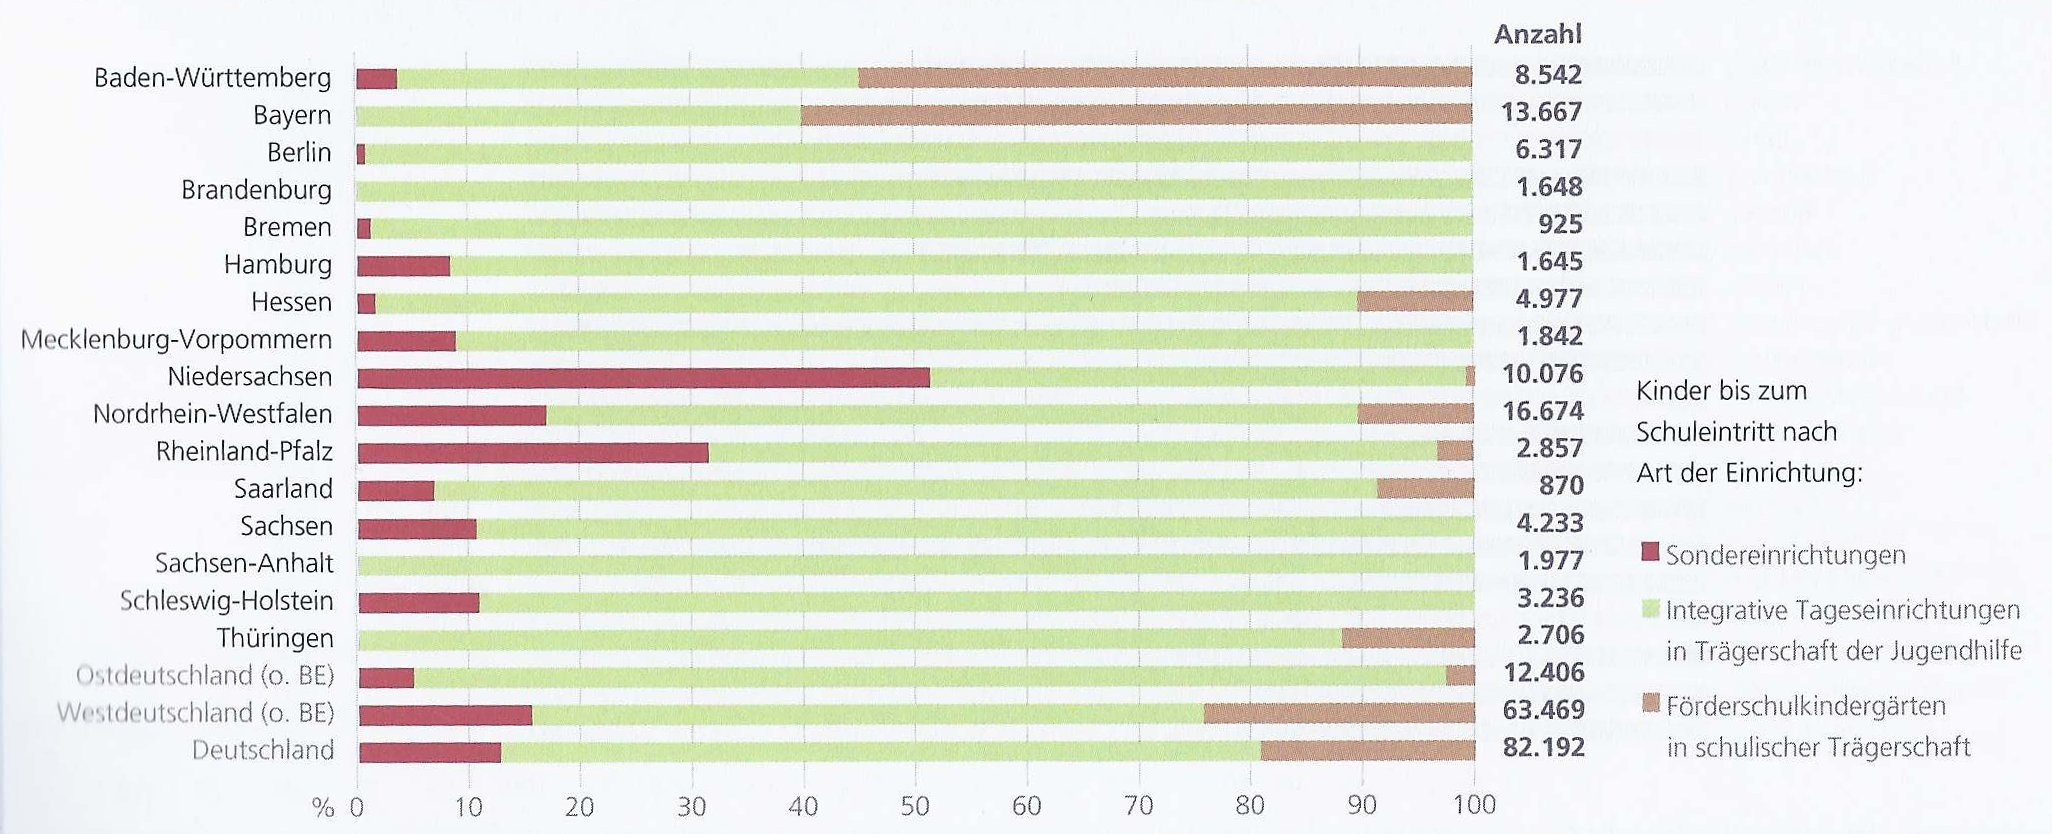
\includegraphics[width=0.95\textwidth]{bilder/bildungsbeteiligung}
  \caption{Bildunsbeteiligung von Kindern mit (drohender) Behinderung nach Art der Einrichtung. Stand: 01.03.2010}
  \label{bild:bildungsbeteiligung}
\end{figure}


\section{Selbstverständnis des Kindergartens unter Berücksichtigung der Trägervielfalt}\label{sec:kitaSelbst}
Aus den voran gestellten Bezugspunkten und ihren Aufgabenbeschreibungen lässt sich anhand von Hugoth (2010, 30) das Selbstverständnis des Kindergartens ableiten. Dieses kann folgendermaßen ausdifferenziert werden:

Der Kindergarten als
\begin{enumerate}
\item erste Stufe des deutschen Bildungssystems,
\item Ergänzung und Unterstützung der Familie,
\item Dienstleister und Teil des Systems der unterstützenden Dienste,
\item Organ des Staates zur Erfüllung seines Wächteramtes und 
\item Ort für alle.
\end{enumerate}

Die inhaltlichen Schwerpunkte der Arbeit im Kindergarten werden nach Hugoth (2010, 19) maßgeblich von der Akzentsetzung der Träger beeinflusst. Die Einrichtungen weisen ein jeweils trägerspezifisches Profil auf, welches sich über die Schwerpunktsetzung der Arbeit hinaus, in der Auswahl des Personals, in der Organisationsform, im Erscheinungsbild nach außen und in der gelebten „Philosophie“ unterscheidet. Dadurch heben sich die Einrichtungen, vor allem die der freien Träger, zum Teil stark voneinander ab. Deutschland hat im Vergleich zu anderen europäischen Ländern die vielfältigste und bunteste Trägerlandschaft. Dies lässt sich durch zweierlei geltende Prinzipien, das des Föderalismus und das der Subsidiarität, erklären. Im SGB VIII~§~3 (vgl. Gastiger~\& Winkler 2009, 312) wird zwischen öffentlichen und freien Trägern unterschieden. Zu den öffentlichen gehören nach §~69 SBG~VIII (ebd., 341) die Landkreise und kreisfreien Städte und die kreisangehörigen Gemeinden. Hugoth (2010, 20) verweist darauf, dass zunehmend mehr Landesgesetze die institutionalisierte Kinderbetreuung in die Hände der Gemeinden vor Ort geben. 

Zu den freien Trägern zählen laut Hugoth: 

\begin{itemize}
\item die kirchlichen Wohlfahrtsverbände Caritas und Diakonie und die katholischen und evangelischen Kirchgemeinden, die mit über 50\,\%
Gesamtanteil (Stand: 2000) das größte Kontingent stellen, 
\item darüber hinaus die Wohlfahrtsverbände wie Arbeiterwohlfahrt, Rotes Kreuz, Paritäischer Wohlfahrtsverband mit ihren Unterorganisationen,
\item Elterninitiativen, Unternehmen und Betriebe sowie
\item gewerbliche Träger\footnote{Auch wenn gewerbliche Träger eigentlich zu den freien Trägern zählen, fallen dem Sprachgebrauch nach alle nicht-staatlichen und nicht-gewerblichen unter die freien Träger.}, zum Beispiel „Little Giants“. Diese zählen zu den teuren, „exklusiven“, bilingualen Kindergärten und werden von Weiß (2010) als „Parallelwelt“ für Privilegierte bezeichnet\footnote{Die Homepage gibt weitere Einblicke in das Konzept von Little Giants: http://www.littlegiants.de}.      
\end{itemize}

Der Erfolg einer Kindertageseinrichtung hängt nach Jansen (2005, 9 f.) im entscheidenden Maße vom Engagement ihres Trägers ab. Erfolg lässt sich danach bemessen, ob der Träger sein Profil zu schärfen in der Lage ist, indem er es an fachlichen, politischen und gegebenenfalls kirchlichen Anforderungen ausrichtet. Ein professionelles Profil begünstigt eine gute Ausgangsposition im Wettbewerb und berufliche Sicherheit. Die an den Trägerverbund gestellten Anforderungen sind sehr komplex und reichen von der wirtschaftlichen Steuerung und Zukunftssicherung der Einrichtung bis hin zu inhaltlichen Fragen. Dem Träger wie auch der Leitung obliegen eine übergeordnete Steuerungsfunktion. Auf eine nähere Ausführung der Aufgabenbereiche des Trägers wird im Rahmen dieser Arbeit verzichtet. Vielmehr soll auf den Zusammenhang hingewiesen werden, dass aufgrund der komplexen Verantwortung des Trägers sein Einfluss auf das Selbstverständnis des Kindergartens entsprechend groß ist. Seine Interessen bilden das übergeordnete Wertesystem der Einrichtung. Darüber hinaus verweist Kock (2004, 13) darauf, dass der Träger auch im Dienste der Gesellschaft steht. Die Trägergröße ist in Verbindung mit dem gesellschaftlichen Einfluss zu bringen. 
Wenn sich die kirchlichen Träger, in der Regel die Gemeinden vor Ort,  die zahlenmäßig stark vertreten sind, zu aktuellen sozialpolitischen oder bildungspolitischen Themen öffentlich äußern oder zukunftsweisende Entscheidungen treffen, sind diese nicht nur für einzelne Familien, sondern für die ganze Gesellschaft von nachhaltiger Bedeutung. Ein aktueller Bezugspunkt ist die Caritas Kampagne 2011 mit dem Leitsatz „Kein Mensch ist perfekt! Behinderte Menschen: Menschen wie du und ich“, die Inklusion zum Jahresthema machte. Anlässlich dieser Kampagne gab es zahlreiche Projekte, öffentliche Positionierungen und Pressemeldungen, die nach Neher (2011) zum Ziel hatten, dass gelingende Inklusion von der gesamten Zivilgesellschaft als Aufgabe anerkannt wird.
   
\subsection{Der Kindergarten als erste Stufe des deutschen Bildungssystems}
Liegle (2006, 6) schreibt, dass im Zuge der Etablierung des Kindergartens als erste Stufe des deutschen Bildungssystems verschiedene Fragen in der Öffentlichkeit diskutiert werden: Ist es die Aufgabe des Kindergartens auf das Lernen in der Schule vorzubereiten? Droht der Kindergarten in Folge dessen zu verschulen? Hugoth (2010, 32) fügt als weiteren Punkt in der Diskussion die Frage nach der Beitragsfreiheit an. Befürworter verweisen auf den Schulbesuch, der ebenfalls ohne Beitragszahlung der Eltern auskommt. Kritiker benennen, dass das System Kindergarten dadurch vor allem für freie Träger nicht mehr bezahlbar sei, weil diese den Fehlbetrag aus dem Mangel der Elternbeiträge nicht kompensieren könnten und sich zurückziehen würden. Das birgt die Gefahr, dass die Vielfalt der Träger- und damit der Kindergartenlandschaft geschmälert und die Wahlfreiheit der Eltern gegebenenfalls unterlaufen werden würde. Dass solcherart Fragen öffentlich unterschiedlich diskutiert werden, beweist die Unterschiedlichkeit der Trägerinteressen, stellvertretend für eine pluralistische Gesellschaft. 

Sowohl im SGB VIII als auch im Bildungsplan wird die wechselseitige Zusammenarbeit von Kindergarten und Schule zur Gewährleistung eines guten Übergangs als wichtige Aufgabe herausgestellt. Liegle (2006,~5~f.) betrachtet es als Selbstverständlichkeit, dass beide Bildungseinrichtungen aufeinander aufbauen, so dass Brüche beim Übergang von der einen zur nächsten Stufe vermieden und eine gewisse Kontinuität gewährleistet wird. Er beschreibt jedoch mit kritischem Blick die politische Tendenz in Deutschland, die Misere des Bildungssystems mit Hilfe einer gezielten Förderung auf die Schule  beheben zu wollen, da die „eigenständige Bildungskultur“ des Kindergartens hervorzuheben sei.
Dass politische Maßnahmen als Folge des PISA-Schocks zu kurz greifen, die den Kindergarten als vorschulische Einrichtung umdefinieren wollen, kann mit Hilfe von empirischen Untersuchungen als nicht wirksam nachgewiesen werden. \footnote{Liegle (2006, 5 f.) weist in diesem Zusammenhang auf Macon hin, der 2002 in einer breit angelegten Studie nachweisen konnte, dass Kinder, die ein stark formalisiertes und strukturiertes Vorschulprogramm besucht hatten, signifikant schlechtere Noten im 6. Schuljahr hatten als die Vergleichsgruppe, die Vorschulprogramme mit Betonung auf selbstinitiierten und spielerischen Lernen besucht hatten. Außerdem verweist Liegle auf eine deutsche Studie von Tietze, die zu den gleichen Ergebnissen kommt und zeigt, dass der Kindergarten am erfolgreichsten ist, der sich auf seinen eigenständigen Bildungsauftrag besinnt und nicht die Schulvorbereitung betont.}

Laut Becker-Stoll (2009, 46) gehört zu den psychischen Grundbedürfnisse eines Kindes neben Autonomie und Kompetenz auch Bindung. Bindung steht für das Bedürfnis, enge zwischenmenschliche Beziehungen einzugehen, sich sicher gebunden zu fühlen und sich innerhalb dieser Interaktion als liebenswert und liebesfähig zu erleben. Ein „verschulter“ Kindergarten, der die Grundlage für eine optimale Förderung, den Zusammenhang von Bindung und Bildung,  missachtet und Lerninhalte statt das Kind und seine Selbsttätigkeit ins Zentrum stellt, wird zu hinterfragen sein. 
Becker-Stoll (2009, 46) fasst die zentralen Kriterien für eine gelingende frühkindliche Bildung zusammen. Danach gilt, dass 
„Kinder als aktive Lerner betrachtet werden,
die pädagogische Fachkraft auf die individuelle Entwicklung des einzelnen Kindes eingeht,
Spielen als wertvolle Aktivität des Kindes verstanden wird und 
Lerngelegenheiten sinnvoll in den Alltag der Kinder und ihre Initiativen eingebunden werden (Becker-Stoll 2009, 46).“
Das heißt, dass entsprechend der Vorgabe des Bildungsplans Mathematik, Naturwissenschaften oder Sprache und Schrift im Kindergarten durchaus Eingang finden sollen, es heißt laut Draude (2006, 34) nur, „nicht auf die Schule [zu] schielen“ und den Kindern die Möglichkeit zu geben, sich diese Bildungsbereiche spielerisch, selbsttätig und mit allen Sinnen zu erschließen. Sie schreibt, dass der Kindergarten am besten auf Schule vorbereiten würde, der dem Kind Gelegenheit gibt, Ausdauer, Konzentrationsfähigkeit, Ausdrucksfähigkeit, Eigenverantwortlichkeit und Gemeinschaftsfähigkeit auszubilden – Kompetenzen, die in der Schule und im Leben gebraucht werden.

Nach Papke (2010) besteht dabei die Gefahr, dass manche Bildungsbereiche, die im Bildungsplan benannt werden, nicht für alle Kinder als gleichermaßen wichtig angesehen werden, zum Beispiel Naturwissenschaften und Mathematik. Aus der Perspektive von Inklusion stellt sie die Fragen, ob Fachkräfte in den Einrichtungen überhaupt davon überzeugt sind, dass alle Kinder in Bezug auf die empfohlenen Bildungsbereiche gleichermaßen angesprochen sind? Gesetzt dem Fall, was muss bei der Gestaltung dieser Bildungsbereiche berücksichtigt werden, damit diese für alle Kinder interessant und individuell nutzbringend sind? Nur durch eine solche angeregte Auseinandersetzung kann „einem Denken in unterschiedlichen 'Bildungsgruppen' [vorgebeugt werden] (Papke 2010).“ 
Ein ergebnisorientiertes statt einem ergebnisoffenen Konzept als Grundlage der Einrichtung, wie es bei „Little Giants“ anzutreffen ist, würde Inklusion ausschließen. 
% Klein (2010, 92 f.) Reduzierung der Lernzeiele auf verwertbare Kompetenzen und Fähigkeiten, die Nutzen und Erfolg bringen -- verwrrtungsorientierte Wissengesellschaft -- Gift für Inklusion und Demokratie.
 
\subsection{Der Kindergarten als Ergänzung der Familie}
% Albers (2011, 116) der Einfluss der Familie auf die kindliche Entwicklung gilt als etwa doppelt so hoch wie der institutionaliserte.
Laut Bock-Famulla~\& Lange (2011, 41) ist die Bildungspartnerschaft zwischen Kindergarten und Eltern von zentraler Bedeutung für die optimale Entwicklung des Kindes im Kindergarten. Jeske (1997, 10) bestätigt ebenfalls, dass, wenn zwischen beiden Lebenswelten positive enge Verbindungen statt krasser Gegensätze bestehen, sich dies positiv auf die Entwicklung auswirken würde. Nagel (2009, 204) verweist auf verschiedene Studien, in denen die Interaktionswirkungen zwischen familiärer und außerfamiliärer Betreuung untersucht wird. Die bisherigen Ergebnisse zeigen, dass Entwicklungs- und Bildungschancen vor allem bei bildungsfernen Familien durch ergänzende Betreuung unterstützt werden können, die Unterstützung jedoch effizienter ist, umso aktiver die Familie unterstützend wirken kann. Es kann davon ausgegangen werden, dass beide Bereiche sich gegenseitig beeinflussen und eine gute Kooperation und Abstimmung mit den Eltern deshalb betont werden muss. Konkrete Vorgaben zur Elternbeteiligung lassen sich in den Bildungsplänen finden, deren Inhalte von Schlecht, Förster, Wellner~\& Mörth (2008, 44) zusammen getragen wurden. Bereits im Zusammenhang mit der Aufnahme des Kindes wird als wichtig angesehen, dass Eltern die Möglichkeit gegeben wird, gemeinsam mit ihrem Kind in der Gruppe zu hospitieren und in Austausch mit der Erzieherin zu treten, um mit der Einrichtung, ihrem Konzept sowie der Gruppe vertraut zu werden. Zur Aufgabe der Erzieherin gehört es familiäre, kulturelle und religiöse Besonderheiten des Kindes zu berücksichtigen und diese in den Alltag einzubeziehen. So genannte „Bildungspartnerschaft“ kann durch regelmäßige Elternabende, jährliche Entwicklungsgespräche und allgemeinen Austausch über die Aktivitäten des Kindes erfolgen. Wünschenswert ist auch, dass die Eltern die Möglichkeit bekommen, sich in die pädagogische Arbeit einzubringen. Durch Elternvertreter und -beiräte können Elterninteressen gebündelt und in gemeinsamen Planungs- und Entscheidungsprozessen berücksichtigt werden. Auch schriftliche Elternbefragung ist ein hilfreiches Instrument, Elterninteressen zu erheben beziehungsweise im Auge zu behalten. 

\subsection{Der Kindergarten als Dienstleister}
Nach Hugoth (2010, 34 f.) hat sich in den letzten Jahren bedingt durch eine kritischere Erwartungshaltung von Seiten der Eltern, des Trägers aber auch der Behörden im Bereich der Kinder- und Jugendhilfe der Kindergarten zu einem Dienstleister entwickelt. An selbigen werden  Fragen gerichtet, ob er in Anbetracht dessen, was er leistet, das wert ist, was in ihn investiert wird und ob die erbrachten Leistungen den Bedürfnissen der Kinder und Familien entsprechen. Zudem verstehen sich Eltern nicht mehr als „Laien“, die ihre Kinder von „Profis“ betreuen lassen, sondern vielmehr als Kunden, die ausgewiesene Dienstleistungen erwarten und wird ihren Erwartungen nicht entsprochen, sich nach anderen Kindergartenplätzen umschauen. Hugoth (2010, 35) verweist auf den Aspekt, dass in vielen Kommunen ein Konkurrenzdruck durch ein Überangebot an Kindergartenplätzen und eine schwindende Kinderzahl entsteht. Das zwingt die Einrichtung ihre Qualität unter Beweis zu stellen, um konkurrenzfähig zu sein. 
Hugoth (2010, 36 f.) verweist jedoch darauf, dass eine Einrichtung, die in Leistungskategorien denkt und stets die Bedarfe des Kunden, also der Eltern, im Blick hat, an ihre Grenzen stoßen wird, da sie auch anderem verpflichtet ist. Verpflichtungen ergeben sich aus gesetzlichen Vorgaben, dem vom Träger vorgegebene Profil und fachlichen Wissen sowie beruflicher Erfahrung, was „das Beste“ für das Kind ist. Diese können mit der Orientierung an den Wünschen und Vorstellungen der Eltern von der Erziehung und Bildung ihrer Kinder kollidieren. Um dem Profil als Erziehungs- und Bildungseinrichtung gerecht zu werden empfehlen Fritz~\& Hugoth (2010, 28 f.) von einer „Dienstleistungsorientierung“ statt einem „Dienstleistungsunternehmen“ zu sprechen. Eine reine Orientierung an Kundenzufriedenheit, wie man es von einem wirtschaftlichen Unternehmen kennt, ist nicht möglich beziehungsweise der Qualität der Einrichtung nicht förderlich. 

\subsection{Der Kindergarten als Organ des Staates zur Erfüllung des Wächteramtes}
Die Aufgabe des Wächteramtes ist gesetzlich klar geregelt. Der Träger ist in der Pflicht diesen Auftrag zu erfüllen, Spielraum bei der Umsetzung gibt es in diesem Fall nicht.
 
Hugoth (2010, 32) verweist darauf, dass das Wächteramt an die Kindertagesstätte übertragen und somit zum Bestandteil ihres Betreuungsauftrags wird. Laut ihm (2010, 33) kann die Umsetzung eines so definierten Betreuungsauftrag zu einem Interrollenkonflikt der Erzieherin führen. Die unterschiedlichen Rollen, in denen sie sich befindet, einerseits Wächter und Anwalt des Kindes, andererseits Partner der Eltern sein, können im Einzelfall zuwider laufen. Transparenz des Kindergartens gegenüber den Eltern sei deshalb laut Hugoth (ebd.) geboten, das heißt konkrete Interessen, Inhalte, Arbeitsweisen und normative Grundlagen des Kindergartens sollten beschrieben und für die Eltern zugänglich gemacht werden. 

Kunkel (2010, 43) zeigt zwischen Leistungen und Eingriffen das Spannungsfeld zwischen präventivem und repressivem Wächteramt auf. Zur Erfüllung dieses Schutzauftrags ist Vernetzungsarbeit notwendig, weshalb der Schutzauftrag von mehreren Institutionen, die Kontakt zum Kind haben, garantiert werden muss.
Die Kinder- und Jugendhilfe befindet sich wie auch die Erzieherinnen in einem Spannungsfeld zwischen Dienstleistung und Schutzauftrag. Das staatliche Wächteramt besteht sowohl aus Leistungen wie Tagesbetreuung und Jugendarbeit, wodurch Familien präventiv unterstützt und ergänzt werden sollen, als auch aus Beratung und Erziehungshilfe bei Defizitlagen. Ist die Schwelle des Gefährdungsrisikos jedoch überschritten, sind Jugendamt und Familiengericht gefordert einzugreifen, um die Gefahr vom Kind abzuwenden. 

\subsection{Der Kindergarten als Ort für alle}\label{OrtFuerAlle}
Nach Bock-Famulla~\& Lange (2011, 9) besuchten im Jahr 2010 in Ostdeutschland über 95\,\% und in Westdeutschland knapp 93\,\% der drei bis sechsjährigen Kinder einen Kindergarten. Wenn nahezu jedes Kind einen Kindergartenplatz in Anspruch nimmt, kann nach Kron (2010, 32 f.) folglich davon ausgegangen werden, dass die Heterogenität\footnote{Nach Prengel (2010, 2) bedeutet „heterogen“ verschieden, anders, plural – bezogen auf die Differenzen zwischen Kindergruppen, bezogen auf gruppeninterne Untergruppen und bezogen auf die Differenzen zwischen einzelnen Kindern, also auf ihre individuelle Einzigartigkeit.}
der Kindergartengruppe die gesellschaftliche Vielfalt repräsentiert, davon ausgenommen jedoch die Zahl der in Sondereinrichtungen betreuten Kinder. Die europäische multikulturelle Gesellschaft zeichnet sich durch immer komplexer werdende Differenzen und eine wachsende gesellschaftliche Vielfalt aus, in der traditionelle Unterscheidungsmerkmale verschwimmen. Speck-Hamdan (2011, 16) nennt als Gründe Migrationsbewegung und Individualisierungsprozesse. Der Kindergarten wird zum Spiegel dieser Vielfalt – „die Welt trifft sich im Kindergarten“\footnote{Buchtitel von Oberhuemer, Soltendieck~\& Ulrich, 2001}.
 
Um das Spektrum an Unterschieden überschaubar zu machen, werden eine Reihe von Kategorien angelegt. Im derzeitigen Interesse der Sozialwissenschaften liegen laut Albers (2011, 37) vor allem die Kategorien Migration, Behinderung, sozialer Hintergrund und Geschlechtszugehörigkeit.
Dabei betrachtet Speck-Hamdan (2011, 16) kritisch, dass, wenn nur ein Unterscheidungsmerkmal untersucht wird, es zu Verkürzungen kommen kann, weil sich Differenzlinien überschneiden und die Individualität eines Menschen gerade dadurch bestimmt wird, dass der Mensch mit mehreren Facetten beschrieben werden kann. Deshalb sind die in den Sozialwissenschaften in den Vordergrund gestellten Facetten bei weitem nicht alle, anhand derer Kinder voneinander unterschieden werden können. Mögliche weitere Kategorien zur Wahrnehmung pluraler Differenzen in einer Kindergartengruppe bestehen hinsichtlich Alter, ethnisch-kultureller Herkunft, Sprache, Glaubensrichtung, Eltern, Geschwister, Familienkultur und Sozialisation, Qualität ihrer Bindungserfahrungen, Bildungsbiografie, Lernumfeld, ökonomischer Lebenslage, Entwicklungsverlauf sowie bisheriger Erfahrungen in gleichaltrigen Gruppen. 

Eine Bestandsaufnahme hinsichtlich der Merkmale Migrationshintergrund, soziale Benachteiligung und Entwicklungserschwernisse schließt sich an, die Antwort auf die Frage geben soll, wer im Kindergarten aufeinander trifft. 

Laut Roth~\& Terhart (2009, 8) hat im Jahre 2008 etwa jedes vierte Kindergartenkind einen Migrationshintergrund, das heißt, es selbst oder mindestens eines seiner Elternteile oder auch eines seiner Großelternteile ist seit der Nachkriegszeit in Deutschland eingewandert. Auch hierbei wird ein großer Ost-West-Unterschied deutlich. In den westdeutschen Bundesländern haben 29\,\% der über Dreijährigen einen Migrationshintergrund, in den ostdeutschen Bundesländern lediglich 6\,\%. Von allen Migrantenkindern besucht nahezu jedes dritte Kind eine Gruppe, die sich wiederum zu mindestens 50\,\% aus Kindern mit Migrationshintergrund zusammensetzt. Bei Kindern mit Migrationshintergrund handelt es sich ebenfalls um eine sehr heterogene Gruppe, über die nur sehr schwer allgemeine Aussagen getroffen werden können. Ein verbindender Aspekt ist die häufige Zwei- oder Mehrsprachigkeit. Unterschiede machen sich fest an den Herkunftsländern, der ethnischen Zugehörigkeit, der Aufenthaltsdauer, dem rechtlichen Status und den Beweggründen der Eltern nach Deutschland zu kommen. Der kulturelle Hintergrund kann nach Albers (2011, 38) nicht ohne Bezugnahme auf Faktoren, wie Geschlecht, sozialer Status, Einkommen, Bildungshintergrund, Religion und Alter gesehen werden. 
 
Was sagt ein Migrationshintergrund über das Kind aus? Laut Roth~\& Terhart (2009, 77~f.) steht der Migrationshintergrund in Korrelation zu Armutsverhältnissen. 
Nach der ISS\footnote{Institut für Sozialarbeit und Sozialpädagogik}-Längsschnittstudie zur Kinderarmut in Deutschland (1997 - 2005) wurde herausgefunden, dass bei der Gruppe der Vorschulkinder die Armutsquote bei Kindern mit Migrationshintergrund mit über 40\,\% mehr als doppelt so hoch ist wie bei den Kindern mit deutschem Pass. Gründe für Einkommensarmut der Familien sind vor allem in Zugangsbarrieren zum Ausbildungs- und Arbeitsmarkt und einem häufig niedrigerem Bildungsniveau der Eltern zu suchen.
Laut Weiß (2010) haben Forschungen ergeben, dass Armut an sich noch kein direktes Risiko für die kindliche Entwicklung darstellt, jedoch die Wahrscheinlichkeit für Entwicklungsgefährdungen erhöht ist. 
Einkommensarmut muss laut ihm (2000, 52 f.) nicht zwingend zu Entwicklungsrisiken wie komplexer Unterversorgung oder zu einem unzureichenden oder schädigenden Erziehungsverhalten seitens der Bezugspersonen führen. Das Entwicklungsrisiko hängt vom Ausmaß der Armut, sowohl von ihrer Dauer als auch von ihrer Komplexität und Intensität und zudem von den Bewältigungsstrategien der betroffenen Familien ab. Bei chronischer Armut besteht ein wesentlich größeres Risiko als bei kürzeren Armutsperioden, da individuelle Handlungsspielräume in zentralen Lebensbereichen eingeengt werden oder verloren gehen.
Vor allem bei chronischer Armut werden laut ihm die betroffenen Menschen nicht selten von der Erwerbsgesellschaft ausgegrenzt und fühlen sich in Folge dessen überflüssig, nutzlos und nicht gebraucht, wodurch Zukunftsperspektiven schwinden und Selbstentwertung und Verunsicherung sich ausbreiten. Wenn Kinder in eine solche familiäre Situation hinein geboren werden, dann ist das Risiko erhöht, dass sie auf Eltern treffen, die nicht die Kraft haben den Aufgaben der Pflege und Erziehung hinreichend nachzukommen und die intuitive und empathische Kompetenzen vermissen lassen, da sie bedrängt von hoher existenzieller Unsicherheit in ihren Alltagsproblemen gefangen sind.   
Grundsätzlich besteht „ein plausibler und auch empirisch nachgewiesener Zusammenhang zwischen soziökonomischen und psychosozialen Bealstungssituationen sowie der kindlichen Entwicklungsgefährdung bis hin zu manifesten Behinderungen“ (Weiß, 2000, 51).
Biedinger (2009, 197) hat die Folgen von Einkommensarmut auf die kognitive Entwicklung, das Sozialverhalten und den Wortschatzumfang von 3 bis 4-jährigen Kindern untersucht. Die Ergebnisse zeigen, dass der Einfluss der Armut auf die kindliche Entwicklung und den Wortschatz, jedoch nicht auf das Sozialverhalten signifikant ist und selbst unter Kontrolle der Bildung der Bezugsperson bestehen bleibt. Es konnte gezeigt werden, dass der häusliche Lern- und Erfahrungsspielraum entscheidenden Einfluss auf die Entwicklung nimmt und bei Familien in Armut als ebenfalls verarmt betrachtet werden kann, genauso wie ihre Entfaltungs- und Bildungsmöglichkeiten und die Förderung ihrer individuellen Neigungen und Fähigkeiten.
 
Da Behinderung nach Albers (2011, 38) aus der Wechselwirkung von funktionalen Beeinträchtigung im Zusammenwirken mit sozialen Faktoren entsteht, ist auch hier ein mehrdimensionaler Blick erforderlich. Kinder mit Behinderung sind im Kindergarten zunächst einmal Kinder mit bestimmten Voraussetzungen, zum Beispiel Hörverlust, Sehbeeinträchtigung oder Down-Syndrom, die sich erschwerend auf ihre Entwicklung und ihr Lernen auswirken. Jeder Diagnose liegt eine Spannweite von leichter bis schwerer Ausprägung zugrunde. Kinder mit Down-Syndrom zum Beispiel haben eine Intelligenzminderung und trotzdem gibt es Kinder unter ihnen, die das Abitur absolvieren und wiederum andere, die kaum beschulbar sind. Zudem können auch mehrere dieser bestimmten Voraussetzungen bei einem Kind vorliegen, was die Gruppe der Kinder mit Behinderung insgesamt zu einer sehr heterogenen Gruppe macht. Sarimski (2012, 10) gibt die Prävalenz für unterschiedliche Formen von Behinderung mit insgesamt drei bis vier Prozent an. Darunter zählt er Kinder mit einer Seh- oder Hörschädigung, Körperbehinderung, Spracherwerbsstörung, Lern- oder geistigen Behinderung oder mit Autismusspektrumsstörung. 
Eine sehr viel größere Gruppe bilden Kinder mit Entwicklungsrückständen ohne erkennbare biologische Beeinträchtigung, Teilleistungsstörungen, Verhaltensauffälligkeiten oder in außergewöhnlichen Belastungssituationen, zum Beispiel Kinder psychisch kranker oder suchtkranker Eltern. Nach Klein (2010, 12) zeigt insgesamt jedes fünfte Kind eine solche Entwicklungsproblematik. 

Zusammenfassend kann nach Kron (2010, 32 f.) festgehalten werden, dass Kinder in Deutschland unter sehr unterschiedlichen Bedingungen aufwachsen, so dass Heterogenität eine soziale Tatsachen ist. In Kapitel \ref{sec:heterogenität} wird die Forschungsinitiative des schweizerischen Kinderarztes Remo H. Largo vorgestellt, in der die Heterogenität der Kinder wissenschaftlich untersucht wird. 
Gemeinsam ist allen Kindern, dass sie Kinder sind und dass sie alle einzigartige Bedürfnisse haben. 
Da die Unterschiedlichkeit der Kinder als reale Ausgangslage anerkannt werden muss, gilt es laut Sarimski (2012, 11) pädagogische Lösungen zu entwickeln, die dieser Vielfalt gerecht werden. Das fokussierte Ziel muss demzufolge lauten, ausnahmslos alle Kinder in gleichermaßen guter Qualität betreuen, erziehen und bilden zu wollen.  


\section{Qualitätsmanagement in Kindertageseinrichtungen}

Die Qualitätsfrage ist heute zu einem wichtigen Kriterium unserer Gesellschaft geworden und umfasst alle Bereiche, einschließlich den Dienstleistungssektor. Laut Esch, Klaudy, Micheel~\& Stöbe-Blossey (2006, 9) ging die Bildungsdebatte Anfang der 90er Jahre Hand in Hand mit der nationalen und internationalen Diskussion über Qualitätsfragen im Elementarbereich. Seit der Erneuerung und Erweiterung des Kinder- und Jugendhilfegesetzes (§§ 22 bis 24a SBG VIII) im Jahr 2004 sind die Träger der Kindertagesstätten zur Qualitätsentwicklung verpflichtet. Eine steigende Qualität soll unter anderem Antwort auf bildungs- und sozialpolitische Herausforderungen geben. Als Beispiel ist der erhöhte Anteil an Kindern mit Migrationshintergrund in Kindergartengruppen zu nennen, der die pädagogische Fachkraft vor neue Aufgaben stellt.
Durch die öffentliche Aufklärung über die Bedeutung des Lernens wurde laut Hugoth (2010, 30 f.) auch der öffentliche Druck erhöht, der sich in den Erwartungen an einen guten Kindergarten ausdrückte, was dieser zu leisten habe und wie dieser beschaffen sein sollte. 
Bemühungen, Qualitätsmerkmale festzulegen und qualitätssichernde Maßnahmen zu etablieren, erfolgten z.B. durch die Implementierung der Bildungspläne oder die 1999 vom Bundesministerium für Familie, Frauen, Senioren und Jugend ins Leben gerufene Nationale Qualitätsinitiative im System der Tageseinrichtungen für Kinder (NQI). 
Die aktuellste Antwort auf die Qualitätsfrage ist die Nationale Untersuchung zur Bidlung, Betreuung und Erziehung in der frühen Kindheit (NUBBEK), deren Ergebnisse erst seit diesem Jahr vorliegen. Durch die gemeinsame Anstrengung von Tietze, Becker-Stoll, Bensel, Eckhardt, Haug-Schnabel, Kalicki, Keller~\& Leyendecker (2012, 4) hat sich die  NUBBEK-Studie zum Ziel gesetzt auf hinreichend großer Datenbasis die Qualität in unserem Früherziehungssystem sowohl bezogen auf die Betreuungsqualität in der Familie als auch im institutionellen Setting zu untersuchen. 
  
\subsection{Pädagogische Qualität und ihre Dimensionen}

Tietze (2004, 406) definiert den Qualitätsbegriffs sehr allgemein, was für ein erstes Herantasten als dienlich empfunden wird: Mit Qualität wird die Beschaffenheit einer Dienstleistung bezeichnet und durch eine Reihe charakteristischer und überprüfbarer Eigenschaften näher beschrieben, welche für den Nutzer der Dienstleistung von Bedeutung sind. In dieser allgemeinen Begriffsbestimmung lassen sich in Bezug auf das Untersuchungsfeld Kindergarten drei Variablen näher bestimmen: \begin{enumerate}
\item Die Dienstleistung als eine pädagogische bezieht sich auf die Trias Betreuung, Bildung und Erziehung.
\item Genutzt wird diese Dienstleistung von den Eltern, den Kinder und den Erzieherinnen.
\item Nach Tietze (2004, 407) wird eine Unterteilung der Eigenschaften in drei Dimensionen als hilfreich erachtet: Strukur-, Orientierungs- und Prozessqualität. Auch die Ergebnisqualität kann nach Behr (2009, 67) als weiteres Unterscheidungskonstrukt festgelegt werden.
\end{enumerate}

Ahnert (2011, 153) verweist darauf, dass das Messen von Qualität institutionalisierter Betreuung ein schwieriges Unterfangen darstellt, da von Seiten der betroffenen Nutzer unterschiedliche Qualitätsvorstellungen zu erwarten wären. Tietze (2004, 406) fügt hinzu, dass dieselben Eigenschaften von den Nutzern möglicherweise unterschiedlich bewertet werden. Aus Sicht der Eltern würde sich die Qualität der Einrichtung beispielsweise an Wohnortnähe und adäquaten Betreuungszeiten -- Merkmale, die mit ihrem Beruf gut vereinbar sind -- bemessen. Dasselbe Qualitätsmerkmal „verlängerte Öffnungszeiten“ würde aus der Perspektive der Erzieherin bedeuten, einen Arbeitsplatz mit Schichtbetrieb und daraus resultierend familienunfreundliche Arbeitszeiten vorzufinden.  

Um Klarheit in die Qualitätsdebatte zu bringen, wurde laut Ahnert (2011, 153 f.) von der National Association for Education of Young Children (NAEYC) schon vor längerer Zeit das Kind und die „Angemessenheit von Betreuungspraktiken in Bezug auf die kindliche Entwicklung“ () ins Zentrum der Debatte gestellt. Wenn nach Tietze (2004, 407) von pädagogischer Qualität gesprochen wird, dann ist ein konkreter Bezug zur kindlichen Entwicklung vorausgesetzt. Pädagogische Qualität ist nur dann gegeben, „wenn diese das körperliche, emotionale, soziale, intellektuelle Wohl sowie die gegenwärtigen und zukünftigen Entwicklungen der Kinder in diesen Bereichen fördert und die Familien in ihrer Betreuungs- und Erziehungsaufgabe untertsützt“ (Tietze 2004, 407). Um pädagogische Qualität zu bestimmen, müssen vorab Qualitätsindikatoren in Bezug auf einen guten Kindergarten unter Perspektive des Kindes und seiner Entwicklungsförderung entwickelt werden. Die Qualität als Ergebnis misst sich dann daran, inwieweit diese Festlegungen in der Praxis umgesetzt werden konnten. Dafür ist eine Evaluation erforderlich. 

Kritisch merken Honig et al. (2004, 13 f.) an, dass die dominierende frühpädagogische Qualitätsdebatte, die wie selbstverständlich auf das Kind und seine Entwicklung sowie auf den Handlungsraum der einzelnen Einrichtung bezogen ist, eine Verengung darstellt. Verengt insofern, dass dabei wichtige Aspekte unberücksichtigt bleiben. Kindergärten sind „soziale Räume“ und als solche in komplexe gesellschaftliche Funktionszusammenhänge und kulturelle Kontexte eingebettet. „Daher sind die Maßstäbe für einen guten Kindergarten nicht nur vielfältig, sondern unvermeidlich strittig; bei genauem Hinsehen weisen sie sogar eine dilemmatische Struktur auf, weil das System der Tageseinrichtungen für Kinder in ein Netz heterogener generalisierter Erwartungshorizonte eingebunden ist. Kindergärten sind entsprechend Schauplatz von Auseinandersetzungen um unterschiedliche Interessen, die mit ungleichen Einflusschancen ausgestattet sind. [...] Kindergärten vermögen ihre Güte also nicht autonom zu bestimmen“, sondern müssen die Differenzen immer wieder austarieren. 
Laut der Autoren sollte der Qualitätsdiskurs von der Frage bestimmt werden, wie sich die unterschiedlichen Erwartungen miteinander vereinbaren lassen.

Die Weiterentwicklung der pädagogischen Arbeit und die Sicherung von Qualität im Kindergarten ist laut Tietze, Dittrich, Grenner, Groot-Wilken, Sommerfeld~\& Viernickel (2004, 16 f.) in der Regel Aufgabe der Leitung. Davon abweichend können Qualitätsbeauftragte als Koordinatoren vom Träger gestellt werden oder aber die Leitung überträgt diese Aufgabe einer Fachkraft aus dem Team. 
Der Gewinn, der in der Anwendung von Qualitätsmanagementverfahren für die Erzieherinnen gesehen wird, ist nach Volkert (2008, 75) ein  wachsendes professionelles Selbstverständnis, da die dynamischen Abläufe, um diese im Sinne einer Optimierung weiterentwickeln zu können, differenziert und reflektiert betrachten werden müssen.

In den folgenden Kapiteln soll geklärt werden, was die vier Dimensionen, Strukur-, Orientierungs-, Prozess- und Ergebnisqualität, beinhalten. Darüber hinaus werden einige Beispiele bestehender Qualitätsstandarts gegeben, auch im Hinblick auf die Optimierung gelingender integrativer Praxis. 

Nach Behr (2009, 14) impliziert pädagogische Qualität im Bezug auf Kinder mit Behinderung stets die Dimension der Inklusion, da durch die Behinderung zugleich die Aufgabe der Einbeziehung und Partizipation gestellt ist. Insofern ist der Qualitätsbegriff im inklusiven Verständnis normativ geprägt. 

\subsection{Strukturqualität}
\label{subsec:Strukturquali}
Unter Strukturqualität werden nach Tietze (2004, 407) Aspekte zusammengefasst, die situationsunabhängig, zeitlich stabil sowie politisch regulierbar sind. Darunter zählen die Fachkraft-Kind-Relation, die Ausbildung, Qualifikation und Bezahlung der pädagogischen Fachkräfte sowie die Gruppengröße, die nach Viernickel~\& Schwarz (2009, 15) als zentrale strukturelle Rahmengrößen eingestuft werden. Zentral deshalb, weil bei diesen ein bedeutsamer Zusammenhang zur kindlichen Entwicklung sowie zu Aspekten der Prozessqualität nachgewiesen werden konnte. Weitere Merkmale sind neben der Gruppengröße auch die Zusammensetzung der Gruppe, der zur Verfügung stehende Raum mit seiner materiellen Ausstattung oder die vorgesehenen Zeiten für mittelbare pädagogische Arbeit\footnote{Neben der direkten Arbeit mit den Kindern gibt es weitere Aufgaben, die ein zusätzliche Zeitkontingente erfordern. Mittelbare pädagogische Arbeit umfasst zum Beispiel Elternarbeit, regelmäßige Dokumentation über gezielte Bildungs- und Entwicklungsförderung, Qualitätssicherung und -entwicklung.}.

Eine Expertise zur Bestimmung der Fachkraft-Kind-Relation zeigt, dass je günstiger diese ausfällt, desto positiver sind die pädagogischen Interaktionen, die bildungsanregenden Impulse, das Wohlbefinden, das Verhalten und die Entwicklung der Kinder. Der Schwellenwert für drei bis sechsjährige, bei dessen Unterschreitung das Wohlbefinden der Kinder gefährdet ist, liegt bei circa acht Kinder auf eine Fachkraft. Die aus wissenschaftlicher Sicht notwendigen Standards werden bei der Mehrzahl der Bundesländer nicht erreicht, so die Ergebnisse von Viernickel~\& Schwarz (2009, 15 f.). Wenn es an Personal und Zeit mangelt, sind „ehrgeizig formulierte Bildungsansprüche“, wie sie in den Bildungsplänen durch Aufgabenbereiche wie „Beobachtung und Dokumentation“, „Sprache und Sprachförderung“, „Zusammenarbeit mit Familien“ formuliert werden, schwer umzusetzen.

In Bezug auf Kinder mit Behinderung können nach Sarimski (2012, 145~f.) Daten anhand einer Elternbefragung (Kobelt Neuhaus 2001) und einer Befragung der pädagogische Fachkräfte (Dichans 1990) gewonnen werden. Aus Sicht der Eltern und der pädagogischen Fachkräfte ergeben sich folgende übereinstimmende Qualitätsstandards im Bereich der Strukturqualität:
 
\begin{itemize}
\item Aus Elternsicht: Gruppenstärke von nicht mehr als 18 Kindern, davon höchstens ein bis zwei Kinder mit Behinderung und zwei Fachkräfte; 

aus der Sicht der Erzieherinnen: Gruppenstärke von maximal 15 Kindern bei nicht mehr als einem Drittel Kindern mit Behinderung und drei Mitarbeitern, davon mindestens zwei Fachkräfte,
\item barrierefreie Zugangsmöglichkeiten und entsprechende Ausstattung mit Materialien, die auf die spezifischen Bedürfnisse der Kinder zugeschnittenen sind, 
\item ausreichend Zeit, in der die Erzieherinnen von der Betreuung der Kinder frei gestellt sind, um sich mit heilpädagogischen Fragen innerhalb und außerhalb des Teams zu befassen, Angebote sowie spezielle Fördermaßnahmen differenziert zu planen und intensive Beratung durch Fachdienste wahrzunehmen
\item Fortbildungsmöglichkeiten.
\end{itemize}

\subsection{Orientierungsqualität}
Nach Tietze (2004, 411) erfordert ein entwicklungsfördernder Umgang mit dem Kind hohe formale und berufsbezogene Qualifikation. Eng im Zusammenhang mit der Ausbildungsqualität der Erzieherinnen steht die Orientierungsqualität. Diese umfasst laut ihm (2004, 407 f.) pädagogische Vorstellungen, Werte und Überzeugungen der Erzieherin. Welches Bild sie vom Kind, aber auch von den Eltern hat, wird ihre pädagogische Arbeit maßgeblich bestimmen. Für gelingende inklusive Bildungsprozesse ist eine Ressourcen orientierte Haltung als Grundvoraussetzung anzusehen. Haltungen und Orientierungen werden in der Ausbildung erworben und in Fortbildungen vertieft, sind aber auch von der Persönlichkeit abhängig. 
Da die Empathiefähigkeit der Erzieherin Voraussetzung für eine sichere Bindungsbeziehung zum Kind ist, sehen Haderlein~\& Sell (2007, 24) die Notwendigkeit, die Frage nach der Persönlichkeit offen zu stellen. Denn, „nicht jeder Mensch ist in der Lage im Prozess der Praxis der Betreuung, Erziehung und Bildung von Kindern aus seiner Person selbst heraus eine hohe Qualität zu entfalten, auch und nicht selten trotz eines hohen Reflexionsgrades auf theoretischem Niveau“ (Haderlein~\& Sell 2007, 24). Anders als die Merkmale der Strukturqualität sind die Rahmengrößen der Orientierungsqualität nicht direkt politisch steuerbar, werden jedoch ebenso als zeitlich stabil angesehen. Oft werden übergeordnete Werte auch vom Träger vorgegeben. Sie werden aber auch von den Mitarbeiterinnen erarbeitet und der Konzeption der Einrichtung unter Beachtung vorhandener Rahmenrichtlinien zugrunde gelegt, so dass eine Verständigungsgrundlage nach innen und außen geschaffen wird. 

\subsection{Prozessqualität}
Zur Prozessqualität zählt „all das, was den konkreten Erfahrungs- und Erlebnisraum des Kindes in der Einrichtung unmittelbar gestaltet und beeinflusst“ (Tietze 2001, 7). Prozessqualität bezieht sich auf den Kindergartenalltag mit seinen Interaktionen und Erfahrungen, die das Kind innerhalb seiner sozialen und räumlichen Umwelt macht. Die Prozessqualität wird als dynamisches Konstrukt bezeichnet, da sie situationsabhängig ist. Die Ergebnisse der NUBBEK-Studie herausgegeben von Tietze et al. (2012, 8) weisen im Bereich der Prozessqualität erhöhte Werte auf, wenn keine Altersmischung vorliegt und wenn offene, das heißt gruppenübergreifende Arbeit stattfindet. Es zeigen sich niedriger Werte, je höher der Anteil an Kindern mit Migrationshintergrund ist. Weiterhin zeigt sich, dass die Prozessqualität entscheidend von den Persönlichkeitsmerkmalen der Erzieherin bestimmt wird. Hierin drückt sich die Abhängigkeit der Prozessqualität von Rahmenbedingungen der Struktur- und Orientierungsqualität aus.   

\subsection{Ergebnisqualität}
Die Ergebnisqualität ist vor allem für die Inklusionsperspektive relevant. Nach Behr (2009, 67) werden unter Ergebnisqualität  wahrnehmbare beziehungsweise messbare Auswirkungen einer Maßnahme verstanden, so dass gezeigt werden kann, ob durch spezifische Maßnahmen Entwicklungsfortschritte bei Kindern mit Entwicklungsgefährdungen beobachtet werden können. Für die Beantwortung dieser Fragen können entwicklungsdiagnostische Testverfahren eingesetzt werden.


\section{Zusammenfassung}

Zusammenfassend kann gesagt werden, dass der Kindergarten ein komplexes Praxisfeld darstellt und als solches einen Teil unserer komplexen Gesellschaft, von deren Einflüssen er nicht getrennt gedacht werden darf. Der Kindergartens als offenes System kennt zahlreiche an ihn gestellte Anforderungen von außen, die teilweise konträr zu den Werten laufen, die für Inklusion stehen. 
Ein solches Beispiel, das einem individualisierten Förderansatz im Weg steht, ist der Bildungsanspruch, dass Kindern im Kindergarten ein festgelegtes Repertoire an Kompetenzen vermittelt werden soll, so dass sie im Hinblick auf den Schuleintritt alle die gleichen und somit optimale Voraussetzung haben. Dadurch ist die Teilhabe von Kindern mit Entwicklungseinschränkungen an regulären Aktivitäten der Gruppe gefährdet (vgl. Göransson 2010, Papke 2010, Haug 2011). Festgehalten werden kann, dass das Aufgabenfeld der frühen Bildung, Erziehung und Betreuung sich dem Kind verantwortet und neben dem familiären Einfluss dafür Sorge trägt, welche Chancen sich für das Kind durch kindbezogene gute Begleitung eröffnen.

Welche umfassenden Bemühungen erforderlich sind, Inklusion im Kindergarten im Rahmen der Möglichkeiten umzusetzen, wird im folgenden Kapitel aufgezeigt. Zuvor aber soll geklärt werden, warum die Umsetzung von Inklusion als wertvolles Ziel im Elementarbereich betrachtet werden kann.
